\documentclass{article}
\usepackage{graphics} 
\usepackage{hyperref}

\author{Kevin Zollicoffer}
\title{Predictive Modeling\\Final Project\\\emph{Direct Mail Fundraising Classification}}
\date{10/07/2013}

\usepackage{Sweave}
\begin{document}
\maketitle
%\tableofcontents
\Sconcordance{concordance:DirectMailPrediction.tex:DirectMailPrediction.Rnw:%
1 8 1 1 0 14 1 1 3 110 0 1 2 2 1 1 3 71 0 1 2 3 1 1 2 1 0 1 1 1 2 1 1 3 %
0 1 2 5 1 1 2 1 0 1 1 58 0 1 2 2 1 1 2 1 0 1 1 7 0 1 2 2 1 1 2 5 0 1 2 %
6 1 1 2 5 0 1 2 10 1 1 2 1 0 1 1 3 0 1 2 2 1 1 2 5 0 1 2 7 1 1 2 36 0 1 %
1 35 0 2 1 6 0 1 2 3 1 1 2 1 0 1 2 2 1 1 2 44 0 1 1 18 0 1 1 19 0 1 2 2 %
1 1 2 5 0 1 2 4 1 1 2 1 0 1 1 35 0 1 1 35 0 2 1 6 0 2 2 45 0 1 1 18 0 1 %
1 19 0 1 2 2 1 1 2 5 0 1 2 4 1 1 2 1 0 1 1 35 0 1 1 35 0 2 1 6 0 1 2 1 %
1 1 2 1 0 1 1 35 0 1 1 35 0 2 1 6 0 2 2 132 0 1 1 19 0 1 1 20 0 1 2 2 1 %
1 2 5 0 1 2 4 1 1 2 1 0 1 1 35 0 1 1 35 0 2 1 6 0 1 2 3 1 1 2 1 0 5 1 %
18 0 1 1 3 0 1 2 2 1 1 2 5 0 1 2 6 1 1 2 5 0 1 2 6 1 1 2 36 0 1 1 27 0 %
1 1 35 0 1 1 23 0 2 1 6 0 1 2 26 1 1 2 6 0 1 1 5 0 1 1 10 0 1 4 4 1 1 2 %
1 0 1 1 5 0 1 3 9 1 1 2 1 0 3 1 12 0 1 2 3129 0 1 3 2 1}


\section*{Introduction}
The RStudio project files and accompanying artifacts, including the tex (Rnw) file that created this PDF, are publicly available on GitHub
\\
\url{https://github.com/zollie/PASS-PredictiveModeling-DirectMailPrediction}

\section*{Preliminaries}
The R code here is broken up into seperate scripts for general reuse and orginization. These are presented here, with full up to date versions available on GitHub

\subsubsection*{data.R}
Contains functions and code to load, clean, and setup the data
\begin{Schunk}
\begin{Sinput}
> source('~/R/PASS/PredictiveModeling/DirectMailPrediction/data.R', 
+        echo=TRUE, max.deparse.length=10000)
\end{Sinput}
\begin{Soutput}
> set.seed(12345)

> getRandomRowNums <- function(dd = getDataRaw(), percent = 0.6) {
+     n <- nrow(dd)
+     a <- sort(sample(1:n, floor(n * percent)))
+     a
+ }

> getDataRaw <- function() {
+     dd <- read.csv("~/R/PASS/PredictiveModeling/DirectMailPrediction/DonorData.csv")
+ }

> getDataClean <- function(dd = getDataRaw()) {
+     dd$Row.Id <- NULL
+     dd$Row.Id. <- NULL
+     dd$row.names <- NULL
+     dd$TARGET_D <- NULL
+     dd
+ }

> getDataWithLevels <- function(dd = getDataClean()) {
+     dd$homeowner.dummy <- factor(dd$homeowner.dummy)
+     dd$gender.dummy <- factor(dd$gender.dummy)
+     dd$INCOME <- factor(dd$INCOME)
+     dd$WEALTH <- factor(dd$WEALTH)
+     dd$TARGET_B <- factor(dd$TARGET_B)
+     dd
+ }

> getNnData <- function(dd = getDataClean()) {
+     dd$WEALTH <- nnNormCol(dd$WEALTH)
+     dd$HV <- nnNormCol(dd$HV)
+     dd$lcmed <- nnNormCol(dd$Icmed)
+     dd$lcavg <- nnNormCol(dd$Icavg)
+     dd$IC15 <- nnNormCol(dd$IC15)
+     dd$NUMPROM <- nnNormCol(dd$NUMPROM)
+     dd$RAMNTALL <- nnNormCol(dd$RAMNTALL)
+     dd$MAXRAMNT <- nnNormCol(dd$MAXRAMNT)
+     dd$LASTGIFT <- nnNormCol(dd$LASTGIFT)
+     dd$totalmonths <- nnNormCol(dd$totalmonths)
+     dd$TIMELAG <- nnNormCol(dd$TIMELAG)
+     dd$AVGGIFT <- nnNormCol(dd$AVGGIFT)
+     dd
+ }

> getNnDataPruned <- function(dd = defaultReducePredictors(getDataClean())) {
+     dd$NUMPROM <- nnNormCol(dd$NUMPROM)
+     dd$RAMNTALL <- nnNormCol(dd$RAMNTALL)
+     dd$MAXRAMNT <- nnNormCol(dd$MAXRAMNT)
+     dd$LASTGIFT <- nnNormCol(dd$LASTGIFT)
+     dd$totalmonths <- nnNormCol(dd$totalmonths)
+     dd$TIMELAG <- nnNormCol(dd$TIMELAG)
+     dd
+ }

> nnNormCol <- function(col) {
+     a <- min(col, na.rm = TRUE)
+     b <- max(col, na.rm = TRUE)
+     c2 <- sapply(col, function(x) {
+         (x - a)/(b - a)
+     })
+     c2
+ }

> getFutureDataRaw <- function() {
+     dd <- read.csv("~/R/PASS/PredictiveModeling/DirectMailPrediction/FutureDonorData.csv")
+ }

> getFutureDataClean <- function(dd = getFutureDataRaw()) {
+     dd$Row.Id <- NULL
+     dd$Row.Id. <- NULL
+     dd$X <- NULL
+     dd$X.1 <- NULL
+     dd$X.2 <- NULL
+     dd$X.3 <- NULL
+     dd$X.4 <- NULL
+     dd$X.5 <- NULL
+     dd$X.6 <- NULL
+     dd
+ }

> getFutureDataWithLevels <- function(dd = getFutureDataClean()) {
+     dd$homeowner.dummy <- factor(dd$homeowner.dummy)
+     dd$gender.dummy <- factor(dd$gender.dummy)
+     dd$INCOME <- factor(dd$INCOME)
+     dd$WEALTH <- factor(dd$WEALTH)
+     dd
+     dd
+ }

> reducePredictors <- function(dd = getDataWithLevels(), 
+     drops) {
+     dd[, !(names(dd) %in% drops)]
+ }

> defaultReducePredictors <- function(dd = getDataWithLevels()) {
+     drops <- c("zipconvert_2", "zipconvert_3", "zipconvert_4", 
+         "zipconvert_5", "WEALTH", "HV", "Icmed", "Icavg", "IC15", 
+         "AVGGIFT")
+     reducePredictors(dd, drops)
+ }

> prices <- matrix(c(0, 0, -0.68, 13 - 0.68), 2, 2)
\end{Soutput}
\end{Schunk}

\subsubsection*{funcs.R}
Contains helper functions and code to build classification tables, charts, calculate lift, etc.  
\begin{Schunk}
\begin{Sinput}
> source('~/R/PASS/PredictiveModeling/DirectMailPrediction/funcs.R', 
+        echo=TRUE, max.deparse.length=10000)
\end{Sinput}
\begin{Soutput}
> buildClassTab <- function(p, p.target, cutoff = 0.5) {
+     require(gmodels)
+     if (is.null(cutoff)) {
+         p.vals = p
+     }
+     else {
+         p.vals <- sapply(p, function(y) {
+             ifelse(y < cutoff, 0, 1)
+         })
+     }
+     CrossTable(p.target, p.vals, type = "SPSS", dnn = c("Actual", 
+         "Predicted"))
+ }

> drawRoc <- function(p, p.target) {
+     require(ROCR)
+     p.rocr <- prediction(p, p.target)
+     p.rocr.roc <- performance(p.rocr, "tpr", "fpr")
+     plot(p.rocr.roc, main = "ROC Curve", colorize = T)
+ }

> drawLift <- function(p, p.target, add = FALSE) {
+     require(ROCR)
+     p.rocr <- prediction(p, p.target)
+     p.rocr.lift <- performance(p.rocr, "lift", "rpp")
+     plot(p.rocr.lift, add = add, main = "Lift Curve", colorize = T)
+ }

> adjustTabForOversamp <- function(ct, target, dnn = c("Actual", 
+     "Predicted")) {
+     t <- ct$t
+     actual.0 <- t[1, 1] + t[1, 2]
+     actual.1 <- t[2, 1] + t[2, 2]
+     prop.0 <- 1 - target
+     n <- target * 100
+     x <- actual.1 * 100/n
+     new.0 <- x * prop.0
+     ct
+     x.0 <- ct$prop.row[1, 1] * new.0
+     x.1 <- ct$prop.row[1, 2] * new.0
+     row1 <- matrix(c(x.0, x.1), 1, 2)
+     row2 <- matrix(c(t[2, 1], t[2, 2]), 1, 2)
+     df <- rbind(row1, row2)
+     CrossTable(df, dnn = dnn)
+ }

> netFromCrossTab <- function(ct, prices) {
+     t <- ct$t
+     x00 <- t[1, 1] * prices[1, 1]
+     x01 <- t[1, 2] * prices[1, 2]
+     x10 <- t[2, 1] * prices[2, 1]
+     x11 <- t[2, 2] * prices[2, 2]
+     sum(x00, x01, x10, x11)
+ }

> buildClassTree <- function(formula, data, minspl, 
+     minbuc) {
+     require(rpart)
+     tree.g <- rpart(formula, data = data, method = "class", minsplit = minspl, 
+         minbucket = minbuc)
+     tree.p <- prune(tree.g, tree.g$cptable[which.min(tree.g$cptable[, 
+         "xerror"]), "CP"])
+     tree.p
+ }
\end{Soutput}
\end{Schunk}


\section*{Data Setup}
Factorized data will be used for Logistic Regression and CART
\begin{Schunk}
\begin{Sinput}
> dd <- getDataWithLevels()
> n <- getRandomRowNums(dd)
> dd.train <- dd[n,]
> dd.test <- dd[-n,]
\end{Sinput}
\end{Schunk}

\section*{Model Building (a)}
\subsection*{Logistic Regression}
Logistic Regression is applied here with varying parameters and predictors used. For each continuos predictor, ROC and Lift curves will be generated to compare the models. 

\subsubsection*{Using all predictors available}
\begin{Schunk}
\begin{Sinput}
> logit <- glm(TARGET_B ~ ., family=binomial("logit"), data=dd.train)
> summary(logit)
\end{Sinput}
\begin{Soutput}
Call:
glm(formula = TARGET_B ~ ., family = binomial("logit"), data = dd.train)

Deviance Residuals: 
    Min       1Q   Median       3Q      Max  
-1.7805  -1.1485  -0.7362   1.1463   2.1338  

Coefficients:
                   Estimate Std. Error z value Pr(>|z|)    
(Intercept)      -1.230e+01  3.032e+02  -0.041   0.9676    
zipconvert_2      1.377e+01  3.032e+02   0.045   0.9638    
zipconvert_3      1.371e+01  3.032e+02   0.045   0.9639    
zipconvert_4      1.359e+01  3.032e+02   0.045   0.9643    
zipconvert_5      1.371e+01  3.032e+02   0.045   0.9639    
homeowner.dummy1  1.003e-01  1.248e-01   0.804   0.4214    
NUMCHLD          -2.880e-01  1.384e-01  -2.080   0.0375 *  
INCOME2           2.473e-01  1.971e-01   1.255   0.2095    
INCOME3           2.626e-01  2.202e-01   1.193   0.2330    
INCOME4           2.696e-01  1.842e-01   1.463   0.1435    
INCOME5           4.806e-01  2.000e-01   2.404   0.0162 *  
INCOME6           4.425e-01  2.426e-01   1.824   0.0681 .  
INCOME7           5.585e-01  2.446e-01   2.283   0.0224 *  
gender.dummy1     8.441e-02  9.826e-02   0.859   0.3903    
WEALTH1           5.375e-01  3.366e-01   1.597   0.1103    
WEALTH2          -1.835e-01  3.401e-01  -0.539   0.5896    
WEALTH3           6.874e-02  3.207e-01   0.214   0.8303    
WEALTH4           9.754e-02  3.364e-01   0.290   0.7718    
WEALTH5           9.023e-02  3.247e-01   0.278   0.7811    
WEALTH6           2.486e-01  3.333e-01   0.746   0.4557    
WEALTH7           2.608e-01  3.417e-01   0.763   0.4452    
WEALTH8           2.230e-01  2.733e-01   0.816   0.4145    
WEALTH9           2.012e-01  3.321e-01   0.606   0.5445    
HV                1.275e-04  8.931e-05   1.427   0.1535    
Icmed             6.478e-04  1.178e-03   0.550   0.5823    
Icavg            -1.050e-03  1.285e-03  -0.817   0.4137    
IC15              2.495e-03  5.825e-03   0.428   0.6684    
NUMPROM           4.976e-03  3.569e-03   1.394   0.1633    
RAMNTALL         -2.677e-04  6.930e-04  -0.386   0.6993    
MAXRAMNT          4.317e-03  7.309e-03   0.591   0.5548    
LASTGIFT         -2.264e-02  1.103e-02  -2.053   0.0401 *  
totalmonths      -5.774e-02  1.303e-02  -4.432 9.34e-06 ***
TIMELAG           6.191e-03  8.838e-03   0.701   0.4836    
AVGGIFT           6.560e-03  1.560e-02   0.420   0.6741    
---
Signif. codes:  0 ‘***’ 0.001 ‘**’ 0.01 ‘*’ 0.05 ‘.’ 0.1 ‘ ’ 1

(Dispersion parameter for binomial family taken to be 1)

    Null deviance: 2595.1  on 1871  degrees of freedom
Residual deviance: 2518.7  on 1838  degrees of freedom
AIC: 2586.7

Number of Fisher Scoring iterations: 12
\end{Soutput}
\end{Schunk}
\paragraph{Prediction}

Prediction using the test data is done with the model and evaluated using ROC and Lift curves. 
\begin{Schunk}
\begin{Sinput}
> logit.pred <- predict(logit, newdata=dd.test, type="response")
> summary(logit.pred)
\end{Sinput}
\begin{Soutput}
     Min.   1st Qu.    Median      Mean   3rd Qu.      Max. 
0.0000009 0.4371000 0.5024000 0.5013000 0.5597000 0.8394000 
\end{Soutput}
\end{Schunk}

\begin{figure}
\begin{center}
\begin{Schunk}
\begin{Sinput}
> drawRoc(logit.pred, dd.test$TARGET_B)
\end{Sinput}
\end{Schunk}
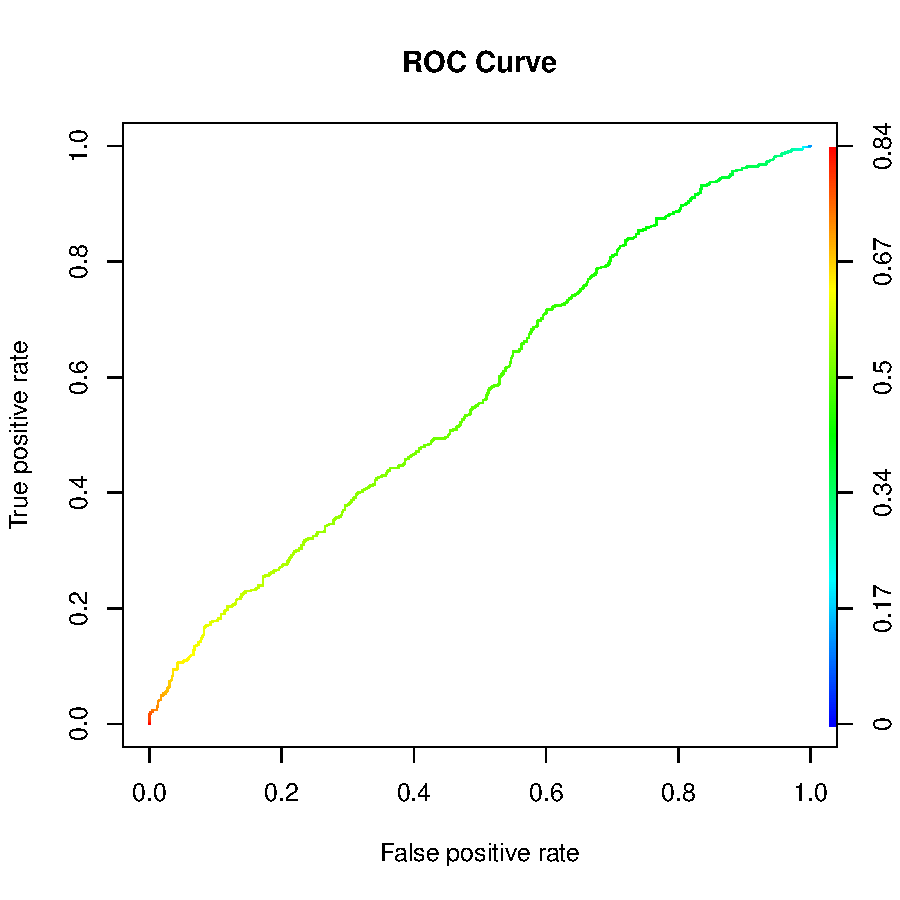
\includegraphics{DirectMailPrediction-006}
\end{center}
\caption{Logistic Regression ROC curve using all predictors}
\label{lr-roc-a}
\end{figure}

\begin{figure}
\begin{center}
\begin{Schunk}
\begin{Sinput}
> drawLift(logit.pred, dd.test$TARGET_B)
\end{Sinput}
\end{Schunk}
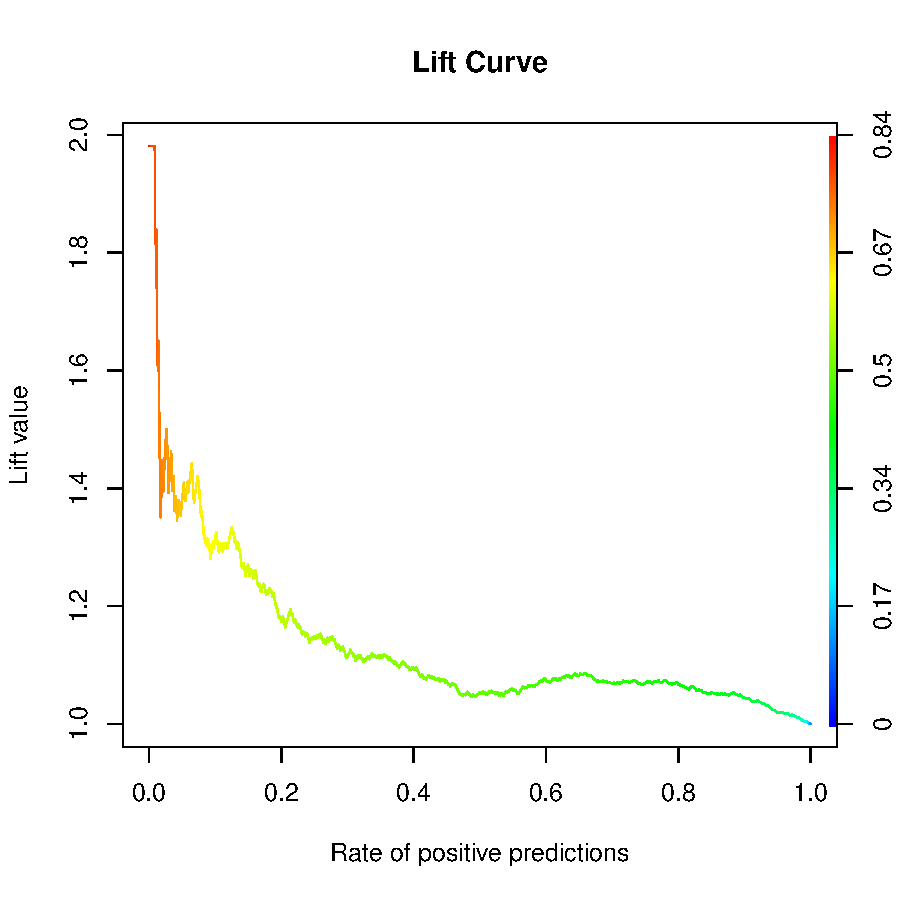
\includegraphics{DirectMailPrediction-007}
\end{center}
\caption{Logistic Regression Lift curve using all predictors}
\label{lr-lift-a}
\end{figure}

\paragraph{Evaluation}
Clearly, this model is not much better than the Naive Rule. 

\paragraph{Subset Selection}
Predictor reduction was attempted but in no case did the ROC curve suggest significantly better results than the Naive Rule. Attempting each predictor one by one also faired no better. The best predictor using Logistic Regression perhaps being LASTGIFT. 

\begin{Schunk}
\begin{Sinput}
> logit.lg <- glm(TARGET_B ~ LASTGIFT, family = binomial("logit"), data = dd.train)
> logit.lg.pred <- predict(logit.lg, newdata=dd.test, type="response")
\end{Sinput}
\end{Schunk}

\begin{figure}
\begin{center}
\begin{Schunk}
\begin{Sinput}
> drawRoc(logit.lg.pred, dd.test$TARGET_B)
\end{Sinput}
\end{Schunk}
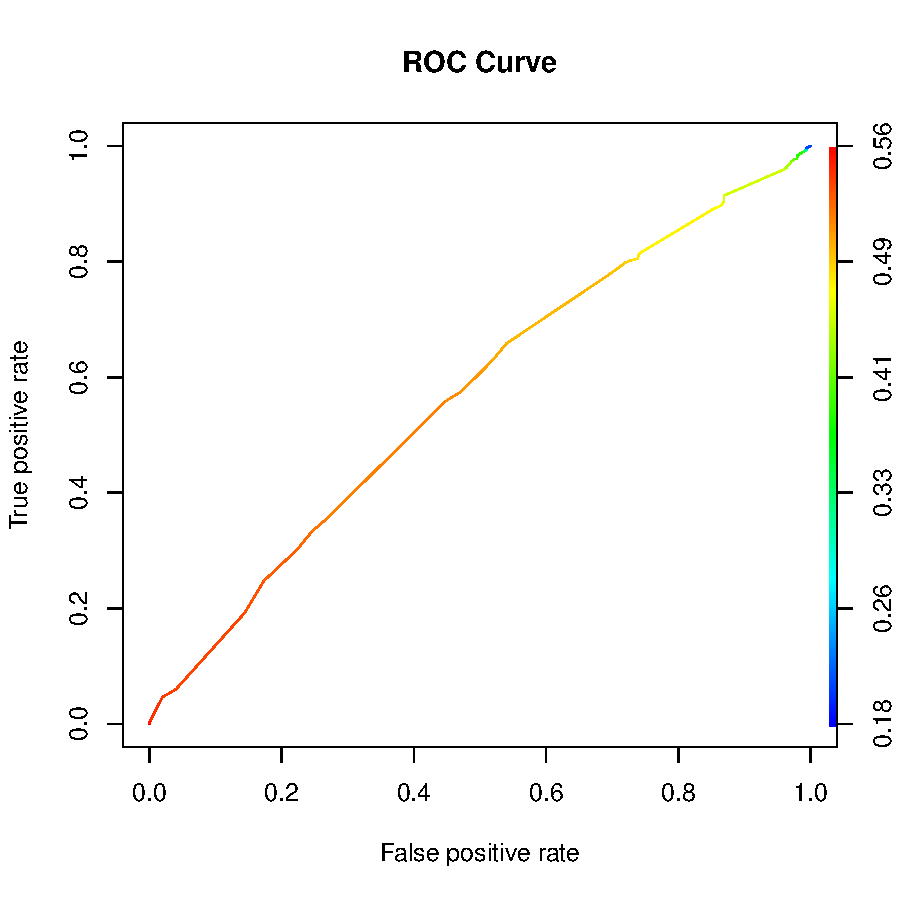
\includegraphics{DirectMailPrediction-009}
\end{center}
\caption{Logistic Regression ROC curve using only LASTGIFT}
\label{lr-roc-b}
\end{figure}

\paragraph{Classification Table and Net Profit}
Classifcation Tables and NetProfit using this model is presented here

\begin{Schunk}
\begin{Sinput}
> ct.logit.lg <- buildClassTab(logit.lg.pred, dd.test$TARGET_B)
\end{Sinput}
\begin{Soutput}
   Cell Contents
|-------------------------|
|                       N |
| Chi-square contribution |
|           N / Row Total |
|           N / Col Total |
|         N / Table Total |
|-------------------------|

 
Total Observations in Table:  1248 

 
             | Predicted 
      Actual |         0 |         1 | Row Total | 
-------------|-----------|-----------|-----------|
           0 |       306 |       312 |       618 | 
             |     4.156 |     3.275 |           | 
             |     0.495 |     0.505 |     0.495 | 
             |     0.556 |     0.447 |           | 
             |     0.245 |     0.250 |           | 
-------------|-----------|-----------|-----------|
           1 |       244 |       386 |       630 | 
             |     4.077 |     3.212 |           | 
             |     0.387 |     0.613 |     0.505 | 
             |     0.444 |     0.553 |           | 
             |     0.196 |     0.309 |           | 
-------------|-----------|-----------|-----------|
Column Total |       550 |       698 |      1248 | 
             |     0.441 |     0.559 |           | 
-------------|-----------|-----------|-----------|
\end{Soutput}
\begin{Sinput}
> ct.logit.lg.a <- adjustTabForOversamp(ct.logit.lg, .051)
\end{Sinput}
\begin{Soutput}
   Cell Contents
|-------------------------|
|                       N |
| Chi-square contribution |
|           N / Row Total |
|           N / Col Total |
|         N / Table Total |
|-------------------------|

 
Total Observations in Table:  12352.94 

 
             | Predicted 
      Actual |             [,1] |             [,2] |        Row Total | 
-------------|------------------|------------------|------------------|
        [1,] |             5804 |             5918 |            11722 | 
             |            0.724 |            0.695 |                  | 
             |            0.495 |            0.505 |            0.949 | 
             |            0.960 |            0.939 |                  | 
             |            0.470 |            0.479 |                  | 
-------------|------------------|------------------|------------------|
        [2,] |              244 |              386 |              630 | 
             |           13.477 |           12.930 |                  | 
             |            0.387 |            0.613 |            0.051 | 
             |            0.040 |            0.061 |                  | 
             |            0.020 |            0.031 |                  | 
-------------|------------------|------------------|------------------|
Column Total |             6048 |             6304 |            12352 | 
             |            0.490 |            0.510 |                  | 
-------------|------------------|------------------|------------------|
\end{Soutput}
\begin{Sinput}
> ct.logit.net <- netFromCrossTab(ct.logit.lg.a, prices)
> ct.logit.net
\end{Sinput}
\begin{Soutput}
[1] 731.0229
\end{Soutput}
\end{Schunk}

\subsection*{CART}
Classification Trees are attempted next

\begin{Schunk}
\begin{Sinput}
> library(rpart.plot)
> tree.a <- buildClassTree(TARGET_B ~ ., dd.train, 3, 1)
> tree.b <- buildClassTree(TARGET_B ~ ., dd.train, 6, 2)
> tree.c <- buildClassTree(TARGET_B ~ ., dd.train, 12, 4)
> summary(tree.a)
\end{Sinput}
\begin{Soutput}
Call:
rpart(formula = formula, data = data, method = "class", minsplit = minspl, 
    minbucket = minbuc)
  n= 1872 

          CP nsplit rel error    xerror       xstd
1 0.12473118      0 1.0000000 1.0397849 0.02324886
2 0.01048387      1 0.8752688 0.9268817 0.02318881

Variable importance
    AVGGIFT    MAXRAMNT    LASTGIFT totalmonths     NUMPROM    RAMNTALL 
         35          25          24           8           5           3 

Node number 1: 1872 observations,    complexity param=0.1247312
  predicted class=0  expected loss=0.4967949  P(node) =1
    class counts:   942   930
   probabilities: 0.503 0.497 
  left son=2 (832 obs) right son=3 (1040 obs)
  Primary splits:
      AVGGIFT     < 9.878676 to the right, improve=16.276920, (0 missing)
      totalmonths < 31.5     to the right, improve=14.088780, (0 missing)
      MAXRAMNT    < 14.5     to the right, improve=13.134850, (0 missing)
      LASTGIFT    < 14.5     to the right, improve=12.963660, (0 missing)
      NUMPROM     < 54.5     to the left,  improve= 8.441558, (0 missing)
  Surrogate splits:
      MAXRAMNT    < 14.5     to the right, agree=0.876, adj=0.720, (0 split)
      LASTGIFT    < 12.5     to the right, agree=0.857, adj=0.679, (0 split)
      totalmonths < 35.5     to the right, agree=0.659, adj=0.232, (0 split)
      NUMPROM     < 24.5     to the left,  agree=0.624, adj=0.155, (0 split)
      RAMNTALL    < 26.5     to the left,  agree=0.596, adj=0.091, (0 split)

Node number 2: 832 observations
  predicted class=0  expected loss=0.4230769  P(node) =0.4444444
    class counts:   480   352
   probabilities: 0.577 0.423 

Node number 3: 1040 observations
  predicted class=1  expected loss=0.4442308  P(node) =0.5555556
    class counts:   462   578
   probabilities: 0.444 0.556 
\end{Soutput}
\begin{Sinput}
> printcp(tree.a)
\end{Sinput}
\begin{Soutput}
Classification tree:
rpart(formula = formula, data = data, method = "class", minsplit = minspl, 
    minbucket = minbuc)

Variables actually used in tree construction:
[1] AVGGIFT

Root node error: 930/1872 = 0.49679

n= 1872 

        CP nsplit rel error  xerror     xstd
1 0.124731      0   1.00000 1.03978 0.023249
2 0.010484      1   0.87527 0.92688 0.023189
\end{Soutput}
\begin{Sinput}
> rsq.rpart(tree.a)
\end{Sinput}
\begin{Soutput}
Classification tree:
rpart(formula = formula, data = data, method = "class", minsplit = minspl, 
    minbucket = minbuc)

Variables actually used in tree construction:
[1] AVGGIFT

Root node error: 930/1872 = 0.49679

n= 1872 

        CP nsplit rel error  xerror     xstd
1 0.124731      0   1.00000 1.03978 0.023249
2 0.010484      1   0.87527 0.92688 0.023189
\end{Soutput}
\end{Schunk}

\begin{figure}
\begin{center}
\begin{Schunk}
\begin{Sinput}
> prp(tree.a)
\end{Sinput}
\end{Schunk}
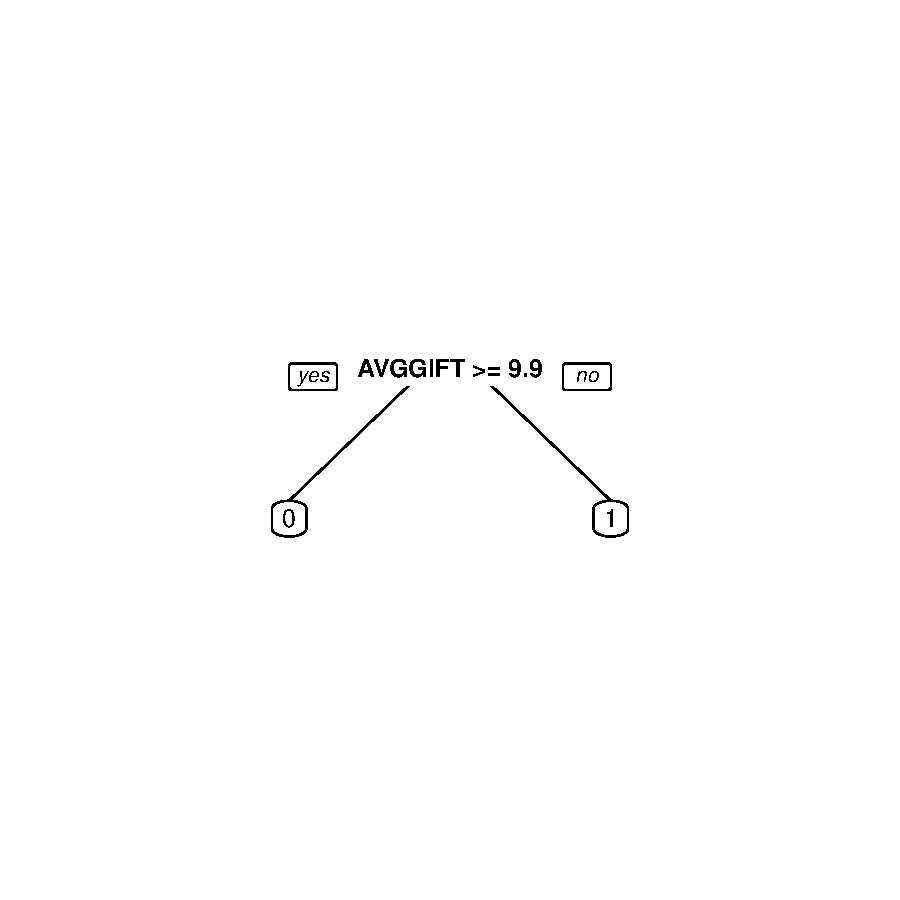
\includegraphics{DirectMailPrediction-012}
\end{center}
\caption{tree.a classification tree}
\label{classt-a}
\end{figure}

\begin{Schunk}
\begin{Sinput}
> tree.a.pred <- predict(tree.a, newdata=dd.test, type="class")
> ct.tree.a <- buildClassTab(tree.a.pred, dd.test$TARGET_B, cutoff=NULL)
\end{Sinput}
\begin{Soutput}
   Cell Contents
|-------------------------|
|                       N |
| Chi-square contribution |
|           N / Row Total |
|           N / Col Total |
|         N / Table Total |
|-------------------------|

 
Total Observations in Table:  1248 

 
             | Predicted 
      Actual |         0 |         1 | Row Total | 
-------------|-----------|-----------|-----------|
           0 |       296 |       322 |       618 | 
             |     2.733 |     2.105 |           | 
             |     0.479 |     0.521 |     0.495 | 
             |     0.545 |     0.457 |           | 
             |     0.237 |     0.258 |           | 
-------------|-----------|-----------|-----------|
           1 |       247 |       383 |       630 | 
             |     2.681 |     2.065 |           | 
             |     0.392 |     0.608 |     0.505 | 
             |     0.455 |     0.543 |           | 
             |     0.198 |     0.307 |           | 
-------------|-----------|-----------|-----------|
Column Total |       543 |       705 |      1248 | 
             |     0.435 |     0.565 |           | 
-------------|-----------|-----------|-----------|
\end{Soutput}
\begin{Sinput}
> ct.tree.a.a <- adjustTabForOversamp(ct.tree.a, .051)
\end{Sinput}
\begin{Soutput}
   Cell Contents
|-------------------------|
|                       N |
| Chi-square contribution |
|           N / Row Total |
|           N / Col Total |
|         N / Table Total |
|-------------------------|

 
Total Observations in Table:  12352.94 

 
             | Predicted 
      Actual |             [,1] |             [,2] |        Row Total | 
-------------|------------------|------------------|------------------|
        [1,] |             5614 |             6108 |            11722 | 
             |            0.485 |            0.438 |                  | 
             |            0.479 |            0.521 |            0.949 | 
             |            0.958 |            0.941 |                  | 
             |            0.455 |            0.494 |                  | 
-------------|------------------|------------------|------------------|
        [2,] |              247 |              383 |              630 | 
             |            9.029 |            8.154 |                  | 
             |            0.392 |            0.608 |            0.051 | 
             |            0.042 |            0.059 |                  | 
             |            0.020 |            0.031 |                  | 
-------------|------------------|------------------|------------------|
Column Total |             5861 |             6491 |            12352 | 
             |            0.475 |            0.525 |                  | 
-------------|------------------|------------------|------------------|
\end{Soutput}
\begin{Sinput}
> net.tree.a <- netFromCrossTab(ct.tree.a.a, prices)
> net.tree.a
\end{Sinput}
\begin{Soutput}
[1] 565.0726
\end{Soutput}
\end{Schunk}

\begin{Schunk}
\begin{Sinput}
> summary(tree.b)
\end{Sinput}
\begin{Soutput}
Call:
rpart(formula = formula, data = data, method = "class", minsplit = minspl, 
    minbucket = minbuc)
  n= 1872 

          CP nsplit rel error    xerror       xstd
1 0.12473118      0 1.0000000 1.0559140 0.02323351
2 0.01048387      1 0.8752688 0.9043011 0.02314150

Variable importance
    AVGGIFT    MAXRAMNT    LASTGIFT totalmonths     NUMPROM    RAMNTALL 
         35          25          24           8           5           3 

Node number 1: 1872 observations,    complexity param=0.1247312
  predicted class=0  expected loss=0.4967949  P(node) =1
    class counts:   942   930
   probabilities: 0.503 0.497 
  left son=2 (832 obs) right son=3 (1040 obs)
  Primary splits:
      AVGGIFT     < 9.878676 to the right, improve=16.276920, (0 missing)
      totalmonths < 31.5     to the right, improve=14.088780, (0 missing)
      MAXRAMNT    < 14.5     to the right, improve=13.134850, (0 missing)
      LASTGIFT    < 14.5     to the right, improve=12.963660, (0 missing)
      NUMPROM     < 54.5     to the left,  improve= 8.441558, (0 missing)
  Surrogate splits:
      MAXRAMNT    < 14.5     to the right, agree=0.876, adj=0.720, (0 split)
      LASTGIFT    < 12.5     to the right, agree=0.857, adj=0.679, (0 split)
      totalmonths < 35.5     to the right, agree=0.659, adj=0.232, (0 split)
      NUMPROM     < 24.5     to the left,  agree=0.624, adj=0.155, (0 split)
      RAMNTALL    < 26.5     to the left,  agree=0.596, adj=0.091, (0 split)

Node number 2: 832 observations
  predicted class=0  expected loss=0.4230769  P(node) =0.4444444
    class counts:   480   352
   probabilities: 0.577 0.423 

Node number 3: 1040 observations
  predicted class=1  expected loss=0.4442308  P(node) =0.5555556
    class counts:   462   578
   probabilities: 0.444 0.556 
\end{Soutput}
\begin{Sinput}
> printcp(tree.b)
\end{Sinput}
\begin{Soutput}
Classification tree:
rpart(formula = formula, data = data, method = "class", minsplit = minspl, 
    minbucket = minbuc)

Variables actually used in tree construction:
[1] AVGGIFT

Root node error: 930/1872 = 0.49679

n= 1872 

        CP nsplit rel error xerror     xstd
1 0.124731      0   1.00000 1.0559 0.023234
2 0.010484      1   0.87527 0.9043 0.023141
\end{Soutput}
\begin{Sinput}
> rsq.rpart(tree.b)
\end{Sinput}
\begin{Soutput}
Classification tree:
rpart(formula = formula, data = data, method = "class", minsplit = minspl, 
    minbucket = minbuc)

Variables actually used in tree construction:
[1] AVGGIFT

Root node error: 930/1872 = 0.49679

n= 1872 

        CP nsplit rel error xerror     xstd
1 0.124731      0   1.00000 1.0559 0.023234
2 0.010484      1   0.87527 0.9043 0.023141
\end{Soutput}
\end{Schunk}

\begin{figure}
\begin{center}
\begin{Schunk}
\begin{Sinput}
> prp(tree.b)
\end{Sinput}
\end{Schunk}
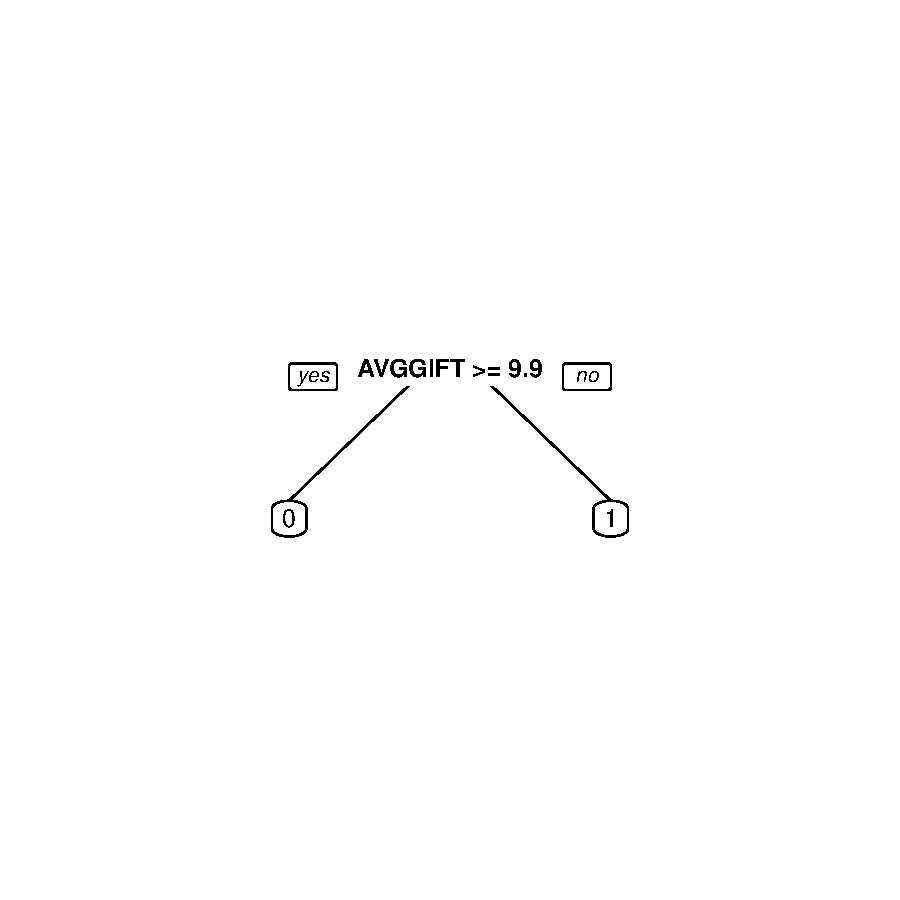
\includegraphics{DirectMailPrediction-015}
\end{center}
\caption{tree.b classification tree}
\label{classt-b}
\end{figure}

\begin{Schunk}
\begin{Sinput}
> tree.b.pred <- predict(tree.b, newdata=dd.test, type="class")
> ct.tree.b <- buildClassTab(tree.b.pred, dd.test$TARGET_B, cutoff=NULL)
\end{Sinput}
\begin{Soutput}
   Cell Contents
|-------------------------|
|                       N |
| Chi-square contribution |
|           N / Row Total |
|           N / Col Total |
|         N / Table Total |
|-------------------------|

 
Total Observations in Table:  1248 

 
             | Predicted 
      Actual |         0 |         1 | Row Total | 
-------------|-----------|-----------|-----------|
           0 |       296 |       322 |       618 | 
             |     2.733 |     2.105 |           | 
             |     0.479 |     0.521 |     0.495 | 
             |     0.545 |     0.457 |           | 
             |     0.237 |     0.258 |           | 
-------------|-----------|-----------|-----------|
           1 |       247 |       383 |       630 | 
             |     2.681 |     2.065 |           | 
             |     0.392 |     0.608 |     0.505 | 
             |     0.455 |     0.543 |           | 
             |     0.198 |     0.307 |           | 
-------------|-----------|-----------|-----------|
Column Total |       543 |       705 |      1248 | 
             |     0.435 |     0.565 |           | 
-------------|-----------|-----------|-----------|
\end{Soutput}
\begin{Sinput}
> ct.tree.b.a <- adjustTabForOversamp(ct.tree.b, .051)
\end{Sinput}
\begin{Soutput}
   Cell Contents
|-------------------------|
|                       N |
| Chi-square contribution |
|           N / Row Total |
|           N / Col Total |
|         N / Table Total |
|-------------------------|

 
Total Observations in Table:  12352.94 

 
             | Predicted 
      Actual |             [,1] |             [,2] |        Row Total | 
-------------|------------------|------------------|------------------|
        [1,] |             5614 |             6108 |            11722 | 
             |            0.485 |            0.438 |                  | 
             |            0.479 |            0.521 |            0.949 | 
             |            0.958 |            0.941 |                  | 
             |            0.455 |            0.494 |                  | 
-------------|------------------|------------------|------------------|
        [2,] |              247 |              383 |              630 | 
             |            9.029 |            8.154 |                  | 
             |            0.392 |            0.608 |            0.051 | 
             |            0.042 |            0.059 |                  | 
             |            0.020 |            0.031 |                  | 
-------------|------------------|------------------|------------------|
Column Total |             5861 |             6491 |            12352 | 
             |            0.475 |            0.525 |                  | 
-------------|------------------|------------------|------------------|
\end{Soutput}
\begin{Sinput}
> net.tree.b <- netFromCrossTab(ct.tree.b.a, prices)
> net.tree.b
\end{Sinput}
\begin{Soutput}
[1] 565.0726
\end{Soutput}
\end{Schunk}


\begin{Schunk}
\begin{Sinput}
> tree.c.pred <- predict(tree.c, newdata=dd.test, type="class")
> ct.tree.c <- buildClassTab(tree.c.pred, dd.test$TARGET_B, cutoff=NULL)
\end{Sinput}
\begin{Soutput}
   Cell Contents
|-------------------------|
|                       N |
| Chi-square contribution |
|           N / Row Total |
|           N / Col Total |
|         N / Table Total |
|-------------------------|

 
Total Observations in Table:  1248 

 
             | Predicted 
      Actual |         0 |         1 | Row Total | 
-------------|-----------|-----------|-----------|
           0 |       225 |       393 |       618 | 
             |     2.158 |     1.063 |           | 
             |     0.364 |     0.636 |     0.495 | 
             |     0.546 |     0.470 |           | 
             |     0.180 |     0.315 |           | 
-------------|-----------|-----------|-----------|
           1 |       187 |       443 |       630 | 
             |     2.117 |     1.043 |           | 
             |     0.297 |     0.703 |     0.505 | 
             |     0.454 |     0.530 |           | 
             |     0.150 |     0.355 |           | 
-------------|-----------|-----------|-----------|
Column Total |       412 |       836 |      1248 | 
             |     0.330 |     0.670 |           | 
-------------|-----------|-----------|-----------|
\end{Soutput}
\begin{Sinput}
> ct.tree.c.a <- adjustTabForOversamp(ct.tree.c, .051)
\end{Sinput}
\begin{Soutput}
   Cell Contents
|-------------------------|
|                       N |
| Chi-square contribution |
|           N / Row Total |
|           N / Col Total |
|         N / Table Total |
|-------------------------|

 
Total Observations in Table:  12352.94 

 
             | Predicted 
      Actual |             [,1] |             [,2] |        Row Total | 
-------------|------------------|------------------|------------------|
        [1,] |             4268 |             7454 |            11722 | 
             |            0.382 |            0.216 |                  | 
             |            0.364 |            0.636 |            0.949 | 
             |            0.958 |            0.944 |                  | 
             |            0.346 |            0.603 |                  | 
-------------|------------------|------------------|------------------|
        [2,] |              187 |              443 |              630 | 
             |            7.115 |            4.014 |                  | 
             |            0.297 |            0.703 |            0.051 | 
             |            0.042 |            0.056 |                  | 
             |            0.015 |            0.036 |                  | 
-------------|------------------|------------------|------------------|
Column Total |             4455 |             7897 |            12352 | 
             |            0.361 |            0.639 |                  | 
-------------|------------------|------------------|------------------|
\end{Soutput}
\begin{Sinput}
> net.tree.c <- netFromCrossTab(ct.tree.c.a, prices)
> net.tree.c
\end{Sinput}
\begin{Soutput}
[1] 388.4416
\end{Soutput}
\end{Schunk}

\begin{Schunk}
\begin{Sinput}
> summary(tree.c)
\end{Sinput}
\begin{Soutput}
Call:
rpart(formula = formula, data = data, method = "class", minsplit = minspl, 
    minbucket = minbuc)
  n= 1872 

          CP nsplit rel error    xerror       xstd
1 0.12473118      0 1.0000000 1.0290323 0.02325577
2 0.01048387      1 0.8752688 0.9193548 0.02317436
3 0.01000000      5 0.8333333 0.9021505 0.02313637

Variable importance
    AVGGIFT    MAXRAMNT    LASTGIFT     NUMPROM totalmonths      INCOME 
         22          17          16          13          11           8 
     WEALTH    RAMNTALL     TIMELAG 
          7           5           2 

Node number 1: 1872 observations,    complexity param=0.1247312
  predicted class=0  expected loss=0.4967949  P(node) =1
    class counts:   942   930
   probabilities: 0.503 0.497 
  left son=2 (832 obs) right son=3 (1040 obs)
  Primary splits:
      AVGGIFT     < 9.878676 to the right, improve=16.276920, (0 missing)
      totalmonths < 31.5     to the right, improve=14.088780, (0 missing)
      MAXRAMNT    < 14.5     to the right, improve=13.134850, (0 missing)
      LASTGIFT    < 14.5     to the right, improve=12.963660, (0 missing)
      NUMPROM     < 54.5     to the left,  improve= 8.441558, (0 missing)
  Surrogate splits:
      MAXRAMNT    < 14.5     to the right, agree=0.876, adj=0.720, (0 split)
      LASTGIFT    < 12.5     to the right, agree=0.857, adj=0.679, (0 split)
      totalmonths < 35.5     to the right, agree=0.659, adj=0.232, (0 split)
      NUMPROM     < 24.5     to the left,  agree=0.624, adj=0.155, (0 split)
      RAMNTALL    < 26.5     to the left,  agree=0.596, adj=0.091, (0 split)

Node number 2: 832 observations,    complexity param=0.01048387
  predicted class=0  expected loss=0.4230769  P(node) =0.4444444
    class counts:   480   352
   probabilities: 0.577 0.423 
  left son=4 (823 obs) right son=5 (9 obs)
  Primary splits:
      NUMPROM     < 118      to the left,  improve=6.056641, (0 missing)
      INCOME      splits as  LLRRRRR,      improve=4.468691, (0 missing)
      Icmed       < 163.5    to the left,  improve=4.277984, (0 missing)
      WEALTH      splits as  RRLRLLRRRR,   improve=3.714286, (0 missing)
      totalmonths < 31.5     to the right, improve=3.479007, (0 missing)
  Surrogate splits:
      MAXRAMNT < 132.5    to the left,  agree=0.99, adj=0.111, (0 split)

Node number 3: 1040 observations
  predicted class=1  expected loss=0.4442308  P(node) =0.5555556
    class counts:   462   578
   probabilities: 0.444 0.556 

Node number 4: 823 observations,    complexity param=0.01048387
  predicted class=0  expected loss=0.4167679  P(node) =0.4396368
    class counts:   480   343
   probabilities: 0.583 0.417 
  left son=8 (161 obs) right son=9 (662 obs)
  Primary splits:
      INCOME splits as  LLRRRRR,      improve=5.633731, (0 missing)
      Icmed  < 158      to the left,  improve=5.307601, (0 missing)
      WEALTH splits as  RRLRLLRRRR,   improve=3.709045, (0 missing)
      Icavg  < 174.5    to the left,  improve=3.161087, (0 missing)
      HV     < 252.5    to the left,  improve=3.051052, (0 missing)
  Surrogate splits:
      IC15 < 54.5     to the right, agree=0.806, adj=0.006, (0 split)

Node number 5: 9 observations
  predicted class=1  expected loss=0  P(node) =0.004807692
    class counts:     0     9
   probabilities: 0.000 1.000 

Node number 8: 161 observations
  predicted class=0  expected loss=0.2981366  P(node) =0.08600427
    class counts:   113    48
   probabilities: 0.702 0.298 

Node number 9: 662 observations,    complexity param=0.01048387
  predicted class=0  expected loss=0.4456193  P(node) =0.3536325
    class counts:   367   295
   probabilities: 0.554 0.446 
  left son=18 (373 obs) right son=19 (289 obs)
  Primary splits:
      totalmonths < 31.5     to the right, improve=4.075566, (0 missing)
      Icmed       < 158      to the left,  improve=4.032445, (0 missing)
      WEALTH      splits as  RRLRLLLLRL,   improve=3.630847, (0 missing)
      IC15        < 7.5      to the left,  improve=3.278974, (0 missing)
      HV          < 251      to the left,  improve=2.809783, (0 missing)
  Surrogate splits:
      LASTGIFT < 14.5     to the right, agree=0.636, adj=0.166, (0 split)
      RAMNTALL < 100.5    to the left,  agree=0.627, adj=0.145, (0 split)
      TIMELAG  < 4.5      to the right, agree=0.612, adj=0.111, (0 split)
      MAXRAMNT < 13.5     to the right, agree=0.594, adj=0.069, (0 split)
      NUMPROM  < 85.5     to the left,  agree=0.591, adj=0.062, (0 split)

Node number 18: 373 observations
  predicted class=0  expected loss=0.3967828  P(node) =0.1992521
    class counts:   225   148
   probabilities: 0.603 0.397 

Node number 19: 289 observations,    complexity param=0.01048387
  predicted class=1  expected loss=0.4913495  P(node) =0.1543803
    class counts:   142   147
   probabilities: 0.491 0.509 
  left son=38 (101 obs) right son=39 (188 obs)
  Primary splits:
      WEALTH   splits as  RRLRLLLLRL,   improve=5.444424, (0 missing)
      MAXRAMNT < 21.5     to the right, improve=3.806479, (0 missing)
      RAMNTALL < 69.5     to the right, improve=3.425653, (0 missing)
      NUMPROM  < 23.5     to the right, improve=2.697049, (0 missing)
      LASTGIFT < 22.5     to the right, improve=2.120607, (0 missing)
  Surrogate splits:
      RAMNTALL    < 124      to the right, agree=0.744, adj=0.267, (0 split)
      NUMPROM     < 40.5     to the right, agree=0.730, adj=0.228, (0 split)
      TIMELAG     < 10.5     to the right, agree=0.696, adj=0.129, (0 split)
      IC15        < 2.5      to the left,  agree=0.664, adj=0.040, (0 split)
      totalmonths < 17.5     to the left,  agree=0.661, adj=0.030, (0 split)

Node number 38: 101 observations
  predicted class=0  expected loss=0.3762376  P(node) =0.05395299
    class counts:    63    38
   probabilities: 0.624 0.376 

Node number 39: 188 observations
  predicted class=1  expected loss=0.4202128  P(node) =0.1004274
    class counts:    79   109
   probabilities: 0.420 0.580 
\end{Soutput}
\begin{Sinput}
> printcp(tree.c)
\end{Sinput}
\begin{Soutput}
Classification tree:
rpart(formula = formula, data = data, method = "class", minsplit = minspl, 
    minbucket = minbuc)

Variables actually used in tree construction:
[1] AVGGIFT     INCOME      NUMPROM     totalmonths WEALTH     

Root node error: 930/1872 = 0.49679

n= 1872 

        CP nsplit rel error  xerror     xstd
1 0.124731      0   1.00000 1.02903 0.023256
2 0.010484      1   0.87527 0.91935 0.023174
3 0.010000      5   0.83333 0.90215 0.023136
\end{Soutput}
\begin{Sinput}
> rsq.rpart(tree.c)
\end{Sinput}
\begin{Soutput}
Classification tree:
rpart(formula = formula, data = data, method = "class", minsplit = minspl, 
    minbucket = minbuc)

Variables actually used in tree construction:
[1] AVGGIFT     INCOME      NUMPROM     totalmonths WEALTH     

Root node error: 930/1872 = 0.49679

n= 1872 

        CP nsplit rel error  xerror     xstd
1 0.124731      0   1.00000 1.02903 0.023256
2 0.010484      1   0.87527 0.91935 0.023174
3 0.010000      5   0.83333 0.90215 0.023136
\end{Soutput}
\end{Schunk}

\begin{figure}
\begin{center}
\begin{Schunk}
\begin{Sinput}
> prp(tree.c)
\end{Sinput}
\end{Schunk}
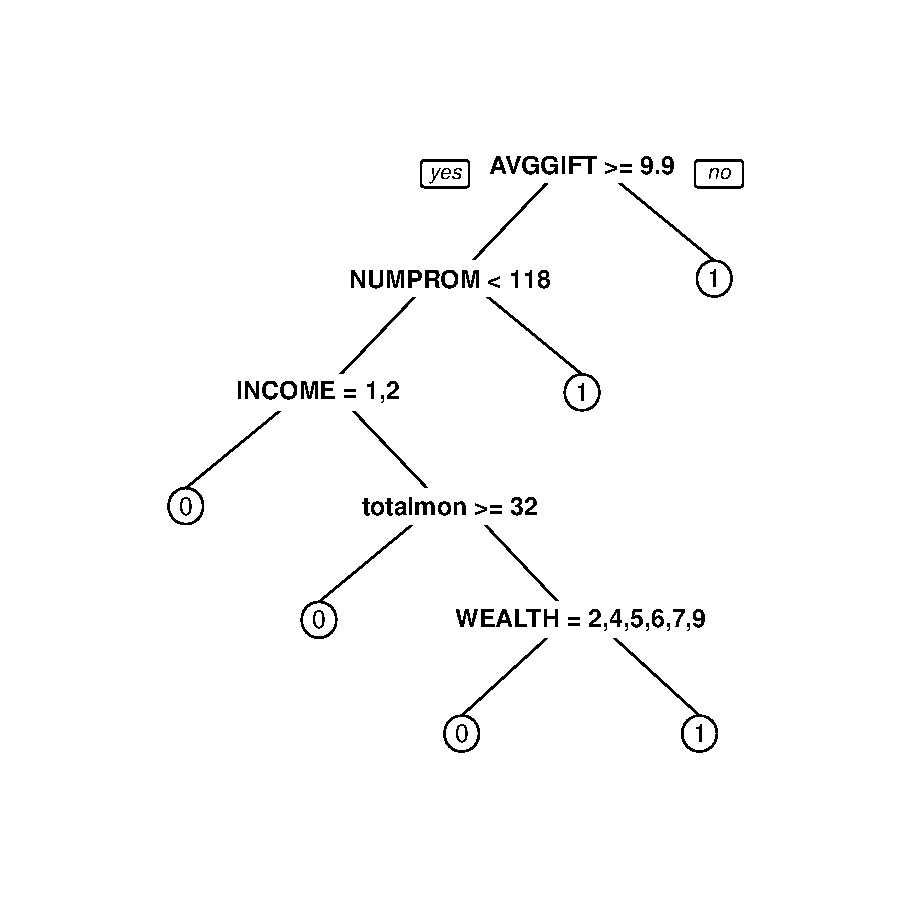
\includegraphics{DirectMailPrediction-019}
\end{center}
\caption{tree.c classification tree}
\label{classt-c}
\end{figure}

\begin{Schunk}
\begin{Sinput}
> tree.c.pred <- predict(tree.c, newdata=dd.test, type="class")
> ct.tree.c <- buildClassTab(tree.c.pred, dd.test$TARGET_B, cutoff=NULL)
\end{Sinput}
\begin{Soutput}
   Cell Contents
|-------------------------|
|                       N |
| Chi-square contribution |
|           N / Row Total |
|           N / Col Total |
|         N / Table Total |
|-------------------------|

 
Total Observations in Table:  1248 

 
             | Predicted 
      Actual |         0 |         1 | Row Total | 
-------------|-----------|-----------|-----------|
           0 |       225 |       393 |       618 | 
             |     2.158 |     1.063 |           | 
             |     0.364 |     0.636 |     0.495 | 
             |     0.546 |     0.470 |           | 
             |     0.180 |     0.315 |           | 
-------------|-----------|-----------|-----------|
           1 |       187 |       443 |       630 | 
             |     2.117 |     1.043 |           | 
             |     0.297 |     0.703 |     0.505 | 
             |     0.454 |     0.530 |           | 
             |     0.150 |     0.355 |           | 
-------------|-----------|-----------|-----------|
Column Total |       412 |       836 |      1248 | 
             |     0.330 |     0.670 |           | 
-------------|-----------|-----------|-----------|
\end{Soutput}
\begin{Sinput}
> ct.tree.c.a <- adjustTabForOversamp(ct.tree.c, .051)
\end{Sinput}
\begin{Soutput}
   Cell Contents
|-------------------------|
|                       N |
| Chi-square contribution |
|           N / Row Total |
|           N / Col Total |
|         N / Table Total |
|-------------------------|

 
Total Observations in Table:  12352.94 

 
             | Predicted 
      Actual |             [,1] |             [,2] |        Row Total | 
-------------|------------------|------------------|------------------|
        [1,] |             4268 |             7454 |            11722 | 
             |            0.382 |            0.216 |                  | 
             |            0.364 |            0.636 |            0.949 | 
             |            0.958 |            0.944 |                  | 
             |            0.346 |            0.603 |                  | 
-------------|------------------|------------------|------------------|
        [2,] |              187 |              443 |              630 | 
             |            7.115 |            4.014 |                  | 
             |            0.297 |            0.703 |            0.051 | 
             |            0.042 |            0.056 |                  | 
             |            0.015 |            0.036 |                  | 
-------------|------------------|------------------|------------------|
Column Total |             4455 |             7897 |            12352 | 
             |            0.361 |            0.639 |                  | 
-------------|------------------|------------------|------------------|
\end{Soutput}
\begin{Sinput}
> net.tree.c <- netFromCrossTab(ct.tree.c.a, prices)
> net.tree.c
\end{Sinput}
\begin{Soutput}
[1] 388.4416
\end{Soutput}
\end{Schunk}

\subsection*{Neural Networks}
The data for a Neural Net needs to be prepared so that the predictors are in the range of [0:1]. Using all predictors resulted in a ROC curve nearly equal to that of the Naive Rule. Therefore, domain knowledge provided by the case writeup was used to prune predictors

\begin{Schunk}
\begin{Sinput}
> library(nnet)
> ddn <- getNnDataPruned()
> n <- getRandomRowNums()
> ddn.train <- ddn[n,]
> ddn.test <- ddn[-n,]
> nn <- nnet(TARGET_B ~ ., data=ddn.train, size=1)
\end{Sinput}
\begin{Soutput}
# weights:  13
initial  value 514.759043 
iter  10 value 467.665761
iter  20 value 467.663370
iter  30 value 466.024357
iter  40 value 463.035281
iter  50 value 462.850599
iter  60 value 462.834356
iter  70 value 460.655083
iter  80 value 460.009379
iter  90 value 457.699723
iter 100 value 455.028110
final  value 455.028110 
stopped after 100 iterations
\end{Soutput}
\begin{Sinput}
> nn.pred <- predict(nn, newdata=ddn.test)
\end{Sinput}
\end{Schunk}

\begin{figure}
\begin{center}
\begin{Schunk}
\begin{Sinput}
> drawRoc(nn.pred, ddn.test$TARGET_B)
\end{Sinput}
\end{Schunk}
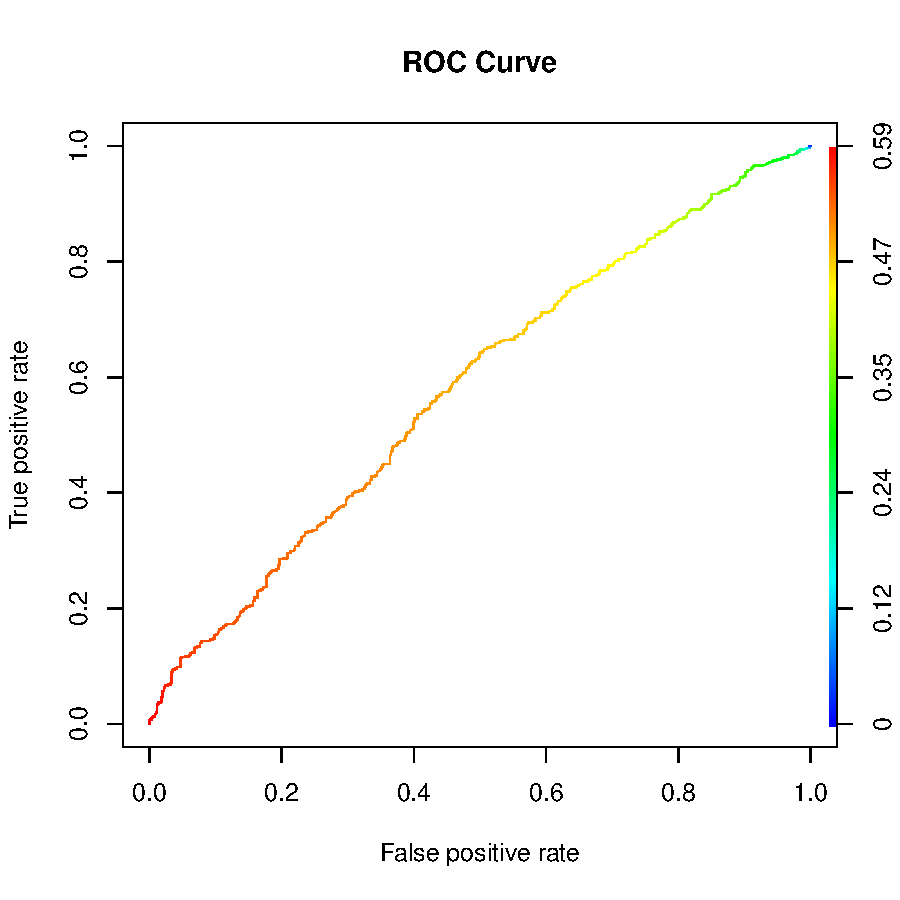
\includegraphics{DirectMailPrediction-022}
\end{center}
\caption{Neural Net ROC curve using Subset Selection}
\label{nn-roc-a}
\end{figure}

\begin{figure}
\begin{center}
\begin{Schunk}
\begin{Sinput}
> drawLift(nn.pred, ddn.test$TARGET_B)
\end{Sinput}
\end{Schunk}
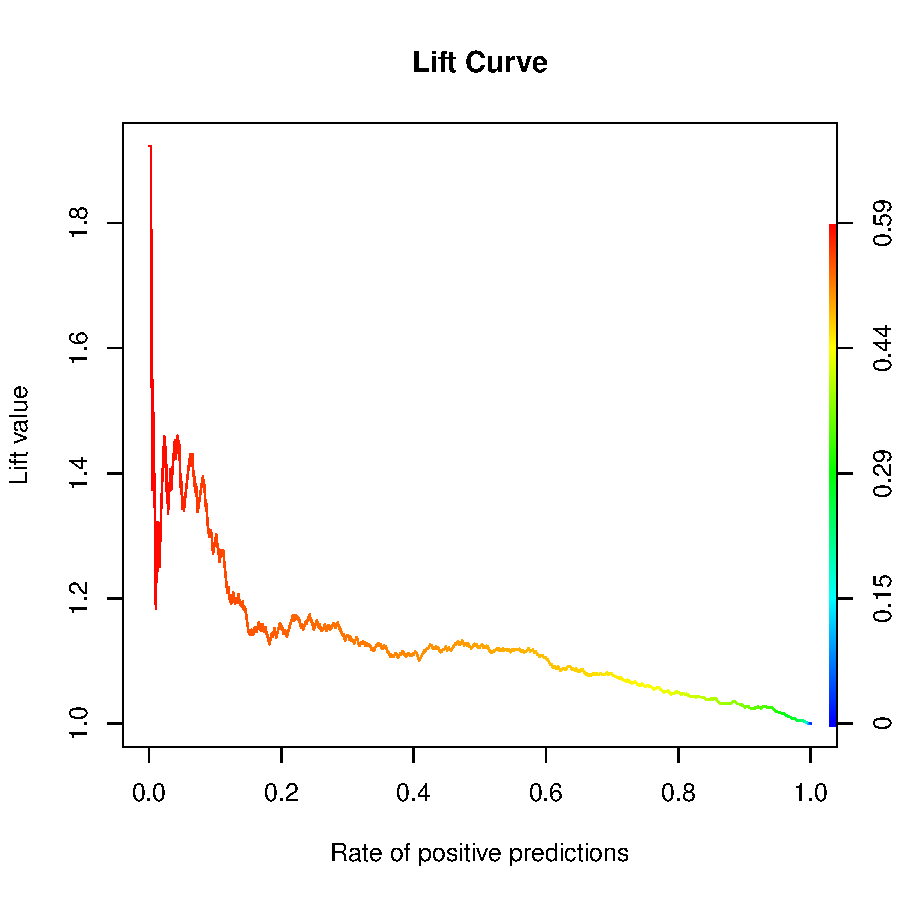
\includegraphics{DirectMailPrediction-023}
\end{center}
\caption{Neural Net Lift curve using Subset Selection}
\label{nn-lift-a}
\end{figure}

\subsubsection*{Classication Table and Net Profit}

\begin{Schunk}
\begin{Sinput}
> nn.ct <- buildClassTab(nn.pred, ddn.test$TARGET_B)
\end{Sinput}
\begin{Soutput}
   Cell Contents
|-------------------------|
|                       N |
| Chi-square contribution |
|           N / Row Total |
|           N / Col Total |
|         N / Table Total |
|-------------------------|

 
Total Observations in Table:  1248 

 
             | Predicted 
      Actual |         0 |         1 | Row Total | 
-------------|-----------|-----------|-----------|
           0 |       361 |       238 |       599 | 
             |     3.781 |     4.512 |           | 
             |     0.603 |     0.397 |     0.480 | 
             |     0.532 |     0.418 |           | 
             |     0.289 |     0.191 |           | 
-------------|-----------|-----------|-----------|
           1 |       318 |       331 |       649 | 
             |     3.489 |     4.164 |           | 
             |     0.490 |     0.510 |     0.520 | 
             |     0.468 |     0.582 |           | 
             |     0.255 |     0.265 |           | 
-------------|-----------|-----------|-----------|
Column Total |       679 |       569 |      1248 | 
             |     0.544 |     0.456 |           | 
-------------|-----------|-----------|-----------|
\end{Soutput}
\begin{Sinput}
> nn.ct
\end{Sinput}
\begin{Soutput}
$t
   y
x     0   1
  0 361 238
  1 318 331

$prop.row
   y
x           0         1
  0 0.6026711 0.3973289
  1 0.4899846 0.5100154

$prop.col
   y
x           0         1
  0 0.5316642 0.4182777
  1 0.4683358 0.5817223

$prop.tbl
   y
x           0         1
  0 0.2892628 0.1907051
  1 0.2548077 0.2652244
\end{Soutput}
\begin{Sinput}
> nn.ct.a <- adjustTabForOversamp(nn.ct, .051)
\end{Sinput}
\begin{Soutput}
   Cell Contents
|-------------------------|
|                       N |
| Chi-square contribution |
|           N / Row Total |
|           N / Col Total |
|         N / Table Total |
|-------------------------|

 
Total Observations in Table:  12725.49 

 
             | Predicted 
      Actual |             [,1] |             [,2] |        Row Total | 
-------------|------------------|------------------|------------------|
        [1,] |             7278 |             4798 |            12076 | 
             |            0.668 |            0.990 |                  | 
             |            0.603 |            0.397 |            0.949 | 
             |            0.958 |            0.935 |                  | 
             |            0.572 |            0.377 |                  | 
-------------|------------------|------------------|------------------|
        [2,] |              318 |              331 |              649 | 
             |           12.434 |           18.413 |                  | 
             |            0.490 |            0.510 |            0.051 | 
             |            0.042 |            0.065 |                  | 
             |            0.025 |            0.026 |                  | 
-------------|------------------|------------------|------------------|
Column Total |             7596 |             5129 |            12725 | 
             |            0.597 |            0.403 |                  | 
-------------|------------------|------------------|------------------|
\end{Soutput}
\begin{Sinput}
> nn.ct.a
\end{Sinput}
\begin{Soutput}
$t
         [,1]     [,2]
[1,] 7278.152 4798.338
[2,]  318.000  331.000

$prop.row
          [,1]      [,2]
[1,] 0.6026711 0.3973289
[2,] 0.4899846 0.5100154

$prop.col
          [,1]       [,2]
[1,] 0.9581367 0.93546926
[2,] 0.0418633 0.06453074

$prop.tbl
           [,1]       [,2]
[1,] 0.57193489 0.37706511
[2,] 0.02498921 0.02601079
\end{Soutput}
\begin{Sinput}
> nn.ct.net <- netFromCrossTab(nn.ct.a, prices)
> nn.ct.net
\end{Sinput}
\begin{Soutput}
[1] 815.0499
\end{Soutput}
\end{Schunk}

\section*{Classification under asymmetric response and cost (b)}
{\it
What is the reasoning behind using weighted sampling to produce training and validation sets with equal numbers of donors and non-donors? Why not use a simple random sample from the original dataset? In this case, is classification accuracy a good performance metric for our purposes of maximizing net profit? If not, how would you determine the best model? Please explain your reasoning.}

\noindent
\newline
If simple sampling were used, the non-responders would drown out the responders due to the 94.9\% rate of non-responders. Using weighted (over) sampling mitigates this phenomonon. 

\noindent
\newline
Classification accuracy is not a good indication of performance as there is a much greater interest in classifiying responders from non-responders.

\noindent
The best model is determined by comparison. Maximzing fund raising is the goal so the model that produces the Classification Table where this is so wins. ROC and Lift curves are used for quick comparison and to rule out models more quickly then rote eximnation of Classification Tables. 

\section*{Calculate Net Profit (c)}
{\it
For each method, calculate the lift of net profit for both the training and validation set based on the actual response rate 5.1\%. Again, the expected donation, given that they are donors, is \$13.00, and the total cost of each mailing is \$0.68.}

\noindent
\newline
This was done for each model above, including adjusting for oversampling

\noindent
\newline
In summary
\begin{Schunk}
\begin{Sinput}
> ct.logit.net
\end{Sinput}
\begin{Soutput}
[1] 731.0229
\end{Soutput}
\begin{Sinput}
> net.tree.a
\end{Sinput}
\begin{Soutput}
[1] 565.0726
\end{Soutput}
\begin{Sinput}
> nn.ct.net
\end{Sinput}
\begin{Soutput}
[1] 815.0499
\end{Soutput}
\begin{Sinput}
> 
> 
\end{Sinput}
\end{Schunk}
\section*{Draw Lift Curves (d)}
{\it
Draw each models net profit lift curve for the validation set onto a single graph. Are there
any models that dominate?}

\begin{Schunk}
\begin{Sinput}
> drawLift(logit.pred, dd.test$TARGET_B)
> drawLift(nn.pred, ddn.test$TARGET_B, add=TRUE)
> #drawLift(tree.a.pred, dd.test$TARGET_B, add=TRUE)
\end{Sinput}
\end{Schunk}
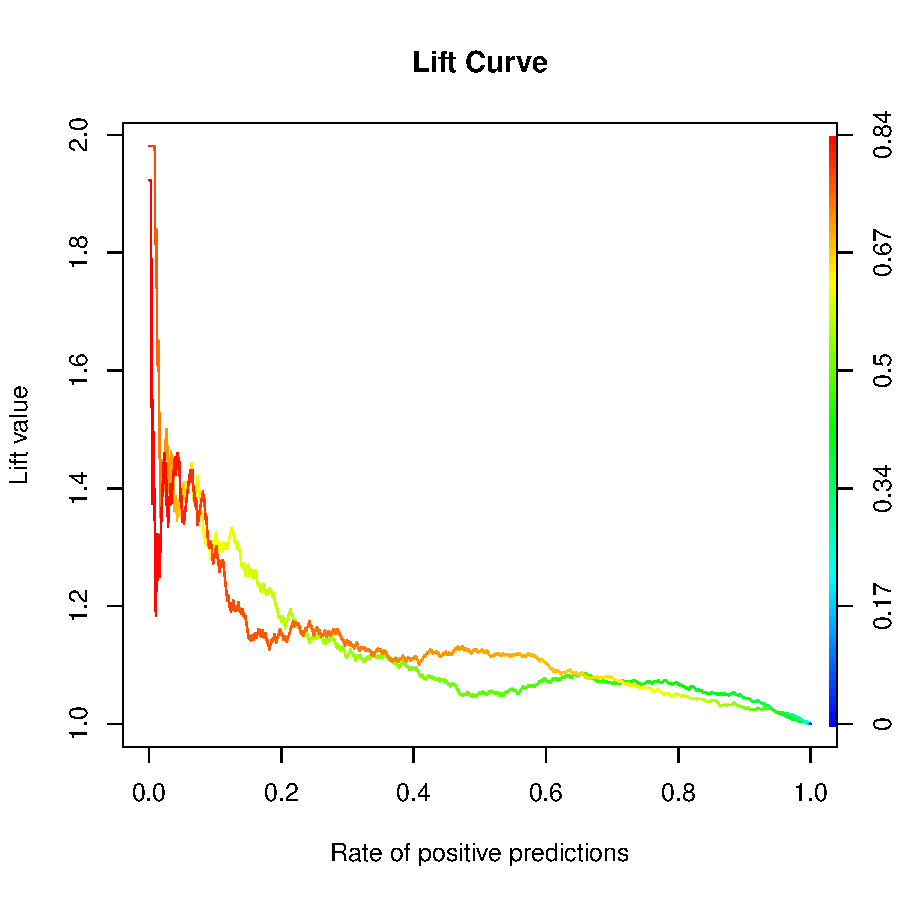
\includegraphics{DirectMailPrediction-026}

\section*{Best Model (e)}
{\it
From your answer in part 2b, what do you think is the best model?}

\noindent
\newline
I choose the Neural Network model as the best in this case. It seems to model the complex relationships between the predcitor variables more accurately, although no model is a clear winner. In this case, it maximizes the fundraising goal. 

\section*{Future Data}
\begin{Schunk}
\begin{Sinput}
> fdd <- getFutureDataClean()
> fdd.nn <- getNnDataPruned(fdd)
> fdd.pred <- predict(nn, newdata=fdd)
> summary(fdd.pred)
\end{Sinput}
\begin{Soutput}
       V1        
 Min.   :0.0000  
 1st Qu.:0.5902  
 Median :0.5902  
 Mean   :0.4944  
 3rd Qu.:0.5902  
 Max.   :0.5902  
 NA's   :1120    
\end{Soutput}
\begin{Sinput}
> fdd.pred
\end{Sinput}
\begin{Soutput}
             [,1]
1    5.902334e-01
2    0.000000e+00
3    5.902334e-01
4    5.902334e-01
5    5.902334e-01
6    5.902334e-01
7    0.000000e+00
8    5.902334e-01
9    5.902334e-01
10   0.000000e+00
11   5.902334e-01
12   5.902334e-01
13   5.902334e-01
14   5.902334e-01
15   5.902334e-01
16   0.000000e+00
17   5.902334e-01
18   5.902334e-01
19   0.000000e+00
20   0.000000e+00
21   5.902334e-01
22   0.000000e+00
23   5.902334e-01
24   0.000000e+00
25   5.902334e-01
26   5.902334e-01
27   5.902334e-01
28   5.902334e-01
29   5.902334e-01
30   5.902334e-01
31   5.902334e-01
32   5.902334e-01
33   0.000000e+00
34   0.000000e+00
35   5.902334e-01
36   5.902334e-01
37   5.902334e-01
38   0.000000e+00
39   5.902334e-01
40   5.902334e-01
41   5.902334e-01
42   5.902334e-01
43   5.902334e-01
44   5.902334e-01
45   5.902334e-01
46   5.902334e-01
47   5.902334e-01
48   5.902334e-01
49   5.902334e-01
50   5.902334e-01
51   5.902334e-01
52   5.902334e-01
53   5.902334e-01
54   5.902334e-01
55   5.902334e-01
56   5.902334e-01
57   5.902334e-01
58   5.902334e-01
59   5.902334e-01
60   5.902334e-01
61   5.902334e-01
62   5.902334e-01
63   5.902334e-01
64   5.902334e-01
65   5.902334e-01
66   5.902334e-01
67   5.902334e-01
68   0.000000e+00
69   5.902334e-01
70   5.902334e-01
71   5.902334e-01
72   5.902334e-01
73   5.902334e-01
74   5.902334e-01
75   5.902334e-01
76   5.902334e-01
77   5.902334e-01
78   5.902334e-01
79   5.902334e-01
80   5.902334e-01
81   5.902334e-01
82   5.852950e-01
83   0.000000e+00
84   5.902334e-01
85   0.000000e+00
86   5.902334e-01
87   5.902334e-01
88   5.902334e-01
89   5.901071e-01
90   5.902334e-01
91   5.902334e-01
92   5.902334e-01
93   5.902334e-01
94   5.902334e-01
95   0.000000e+00
96   5.902334e-01
97   5.902334e-01
98   5.902334e-01
99   5.902334e-01
100  0.000000e+00
101  0.000000e+00
102  5.902334e-01
103  0.000000e+00
104  0.000000e+00
105  5.902334e-01
106  5.902334e-01
107  5.902334e-01
108  5.902334e-01
109  5.902334e-01
110  5.902334e-01
111  5.902334e-01
112  5.902334e-01
113  5.182083e-01
114  5.902334e-01
115  5.902334e-01
116  0.000000e+00
117  5.902334e-01
118  5.902334e-01
119  5.902334e-01
120  5.902334e-01
121  5.902334e-01
122  5.902334e-01
123  5.902334e-01
124  5.902334e-01
125  5.902334e-01
126  5.902334e-01
127  5.902334e-01
128  0.000000e+00
129  0.000000e+00
130  5.902334e-01
131  5.902334e-01
132  0.000000e+00
133  5.902334e-01
134  5.902334e-01
135  5.902334e-01
136  5.902334e-01
137  5.902334e-01
138  5.902334e-01
139  5.902334e-01
140  5.902334e-01
141  5.902334e-01
142  5.902334e-01
143  5.902334e-01
144  5.902334e-01
145  0.000000e+00
146  0.000000e+00
147  5.902334e-01
148  5.902334e-01
149  5.902334e-01
150  5.902334e-01
151  5.902334e-01
152  5.902334e-01
153  5.902334e-01
154  0.000000e+00
155  5.902334e-01
156  5.902334e-01
157  5.902334e-01
158  0.000000e+00
159  5.902334e-01
160  5.902334e-01
161  5.902334e-01
162  5.902334e-01
163  5.902334e-01
164  5.902334e-01
165  5.902334e-01
166  5.902334e-01
167  5.902334e-01
168  5.902334e-01
169  5.902334e-01
170  5.902334e-01
171  5.902334e-01
172  5.902334e-01
173  5.902334e-01
174  5.902334e-01
175  5.902334e-01
176  0.000000e+00
177  5.902334e-01
178  5.902334e-01
179  5.902334e-01
180  0.000000e+00
181  5.902334e-01
182  5.902334e-01
183  5.902334e-01
184  5.902334e-01
185  5.902334e-01
186  5.902334e-01
187  0.000000e+00
188  5.902334e-01
189  5.902334e-01
190  5.902334e-01
191  5.902334e-01
192  5.902334e-01
193  0.000000e+00
194  5.902334e-01
195  5.900551e-01
196  5.902334e-01
197  5.902334e-01
198  5.902334e-01
199  5.902334e-01
200  0.000000e+00
201  5.902334e-01
202  5.902334e-01
203  5.902334e-01
204  0.000000e+00
205  5.902334e-01
206  5.902334e-01
207  5.902334e-01
208  5.902334e-01
209  5.902334e-01
210  5.902334e-01
211  5.902334e-01
212  5.902334e-01
213  5.902334e-01
214  5.902334e-01
215  5.902334e-01
216  5.902334e-01
217  5.902334e-01
218  0.000000e+00
219  5.902334e-01
220  5.902334e-01
221  5.902334e-01
222  5.902334e-01
223  5.902334e-01
224  5.902334e-01
225  5.902334e-01
226  5.902334e-01
227  5.902334e-01
228  5.902334e-01
229  5.902334e-01
230  0.000000e+00
231  5.902334e-01
232  5.902334e-01
233  0.000000e+00
234  0.000000e+00
235  5.902334e-01
236  5.902334e-01
237  5.902334e-01
238  0.000000e+00
239  5.902334e-01
240  5.898997e-01
241  5.902334e-01
242  5.902334e-01
243  0.000000e+00
244  0.000000e+00
245  5.902334e-01
246  5.902334e-01
247  5.902334e-01
248  5.902334e-01
249  5.902334e-01
250  5.902334e-01
251  0.000000e+00
252  5.902334e-01
253  5.902334e-01
254  5.902334e-01
255  0.000000e+00
256  5.902334e-01
257  5.902334e-01
258  5.902334e-01
259  5.902334e-01
260  0.000000e+00
261  0.000000e+00
262  5.902334e-01
263  0.000000e+00
264  5.902334e-01
265  5.902334e-01
266  5.902334e-01
267  5.902334e-01
268  5.902334e-01
269  0.000000e+00
270  5.491238e-01
271  5.902334e-01
272  5.902334e-01
273  5.902334e-01
274  5.902334e-01
275  5.902334e-01
276  5.902334e-01
277  0.000000e+00
278  5.902334e-01
279  5.902334e-01
280  5.902334e-01
281  0.000000e+00
282  5.902334e-01
283  5.902334e-01
284  5.902334e-01
285  5.902334e-01
286  5.902334e-01
287  5.902334e-01
288  5.902113e-01
289  5.902334e-01
290  0.000000e+00
291  5.902334e-01
292  5.902334e-01
293  5.902334e-01
294  5.902334e-01
295  5.902334e-01
296  0.000000e+00
297  5.902334e-01
298  5.902334e-01
299  5.902334e-01
300  0.000000e+00
301  5.902334e-01
302  5.902334e-01
303  5.902334e-01
304  5.902334e-01
305  5.902334e-01
306  5.902334e-01
307  5.902334e-01
308  0.000000e+00
309  5.902334e-01
310  5.902334e-01
311  0.000000e+00
312  0.000000e+00
313  0.000000e+00
314  5.902334e-01
315  5.902334e-01
316  0.000000e+00
317  5.902334e-01
318  5.902334e-01
319  5.902334e-01
320  5.902334e-01
321  5.902334e-01
322  5.902334e-01
323  5.902334e-01
324  5.902334e-01
325  5.902334e-01
326  5.902334e-01
327  5.902334e-01
328  5.902334e-01
329  5.902334e-01
330  5.902334e-01
331  0.000000e+00
332  5.902334e-01
333  5.902334e-01
334  0.000000e+00
335  5.902334e-01
336  5.902334e-01
337  5.902334e-01
338  5.902334e-01
339  5.902334e-01
340  5.902334e-01
341  5.902334e-01
342  5.902334e-01
343  5.902334e-01
344  5.888828e-01
345  5.902334e-01
346  5.902334e-01
347  0.000000e+00
348  0.000000e+00
349  5.902334e-01
350  5.902334e-01
351  5.902334e-01
352  5.902334e-01
353  5.902334e-01
354  5.902334e-01
355  5.902334e-01
356  0.000000e+00
357  5.902334e-01
358  0.000000e+00
359  5.900311e-01
360  5.902334e-01
361  5.902334e-01
362  0.000000e+00
363  5.902334e-01
364  5.902334e-01
365  5.902334e-01
366  5.902334e-01
367  5.902334e-01
368  5.902334e-01
369  5.902334e-01
370  0.000000e+00
371  5.902334e-01
372  0.000000e+00
373  0.000000e+00
374  5.902334e-01
375  5.902334e-01
376  5.902334e-01
377  5.902334e-01
378  5.902334e-01
379  5.902334e-01
380  5.902334e-01
381  5.902334e-01
382  5.902334e-01
383  5.902334e-01
384  5.902334e-01
385  5.902334e-01
386  5.902334e-01
387  5.902334e-01
388  5.902334e-01
389  0.000000e+00
390  0.000000e+00
391  5.902334e-01
392  0.000000e+00
393  0.000000e+00
394  5.902334e-01
395  5.902334e-01
396  0.000000e+00
397  5.902334e-01
398  5.902334e-01
399  0.000000e+00
400  5.902334e-01
401  0.000000e+00
402  0.000000e+00
403  0.000000e+00
404  5.902334e-01
405  5.902334e-01
406  5.902334e-01
407  5.902334e-01
408  5.902334e-01
409  5.902334e-01
410  5.902334e-01
411  5.902334e-01
412  5.902334e-01
413  0.000000e+00
414  0.000000e+00
415  5.902334e-01
416  5.902334e-01
417  5.902334e-01
418  0.000000e+00
419  5.902334e-01
420  0.000000e+00
421  0.000000e+00
422  0.000000e+00
423  0.000000e+00
424  5.902334e-01
425  5.902334e-01
426  5.902334e-01
427  5.902334e-01
428  5.902334e-01
429  5.902334e-01
430  5.902334e-01
431  5.902334e-01
432  2.284777e-03
433  5.902334e-01
434  5.902334e-01
435  5.902334e-01
436  0.000000e+00
437  0.000000e+00
438  5.902334e-01
439  5.902334e-01
440  5.902334e-01
441  5.902334e-01
442  0.000000e+00
443  5.902334e-01
444  5.902334e-01
445  5.902334e-01
446  0.000000e+00
447  5.902334e-01
448  5.902334e-01
449  5.902334e-01
450  0.000000e+00
451  5.902334e-01
452  5.902334e-01
453  5.902334e-01
454  5.902034e-01
455  5.902334e-01
456  5.902334e-01
457  2.611605e-01
458  5.902334e-01
459  0.000000e+00
460  5.902334e-01
461  5.902334e-01
462  5.902334e-01
463  5.902334e-01
464  5.902334e-01
465  5.902334e-01
466  5.902334e-01
467  5.902334e-01
468  5.902334e-01
469  0.000000e+00
470  0.000000e+00
471  5.902334e-01
472  5.902334e-01
473  5.902334e-01
474  5.902334e-01
475  5.902334e-01
476  5.902334e-01
477  5.902334e-01
478  5.902334e-01
479  0.000000e+00
480  5.902334e-01
481  5.902334e-01
482  5.902334e-01
483  5.902334e-01
484  5.902334e-01
485  5.902334e-01
486  5.902334e-01
487  5.902334e-01
488  5.902334e-01
489  5.902334e-01
490  0.000000e+00
491  0.000000e+00
492  5.902334e-01
493  5.902334e-01
494  5.902334e-01
495  5.902334e-01
496  0.000000e+00
497  5.902334e-01
498  5.902334e-01
499  5.902334e-01
500  5.902334e-01
501  5.902334e-01
502  5.902334e-01
503  5.902334e-01
504  5.902334e-01
505  5.902334e-01
506  5.902334e-01
507  5.577281e-01
508  5.902334e-01
509  5.902334e-01
510  5.902334e-01
511  5.902334e-01
512  5.902334e-01
513  0.000000e+00
514  5.902334e-01
515  5.902334e-01
516  5.902334e-01
517  0.000000e+00
518  5.902334e-01
519  5.902334e-01
520  5.902334e-01
521  5.902334e-01
522  5.902334e-01
523  5.902334e-01
524  5.902334e-01
525  0.000000e+00
526  4.326627e-01
527  2.739410e-01
528  0.000000e+00
529  5.902334e-01
530  5.902334e-01
531  0.000000e+00
532  0.000000e+00
533  5.902334e-01
534  5.902334e-01
535  5.902334e-01
536  5.902334e-01
537  5.902334e-01
538  5.901892e-01
539  0.000000e+00
540  5.902334e-01
541  5.902334e-01
542  5.902334e-01
543  5.902334e-01
544  5.902334e-01
545  5.902334e-01
546  5.902334e-01
547  5.902012e-01
548  0.000000e+00
549  5.902334e-01
550  5.902334e-01
551  5.902334e-01
552  5.902334e-01
553  5.902334e-01
554  5.902334e-01
555  5.902334e-01
556  5.902334e-01
557  5.902334e-01
558  5.902334e-01
559  5.902334e-01
560  0.000000e+00
561  5.902223e-01
562  5.902334e-01
563  0.000000e+00
564  0.000000e+00
565  5.902334e-01
566  5.902334e-01
567  5.902334e-01
568  5.902334e-01
569  0.000000e+00
570  5.902334e-01
571  5.902334e-01
572  5.902334e-01
573  5.902334e-01
574  5.902334e-01
575  5.902334e-01
576  5.902334e-01
577  5.902334e-01
578  5.902334e-01
579  5.902334e-01
580  5.902334e-01
581  5.902334e-01
582  5.890666e-01
583  5.902334e-01
584  0.000000e+00
585  5.902334e-01
586  5.902334e-01
587  5.902334e-01
588  5.902334e-01
589  5.902334e-01
590  5.902334e-01
591  5.902334e-01
592  5.902334e-01
593  5.902334e-01
594  5.902334e-01
595  5.902334e-01
596  5.902334e-01
597  0.000000e+00
598  0.000000e+00
599  5.902334e-01
600  0.000000e+00
601  5.902334e-01
602  5.902334e-01
603  5.902334e-01
604  5.869158e-01
605  5.902334e-01
606  5.902334e-01
607  5.902334e-01
608  5.902334e-01
609  5.902334e-01
610  5.902334e-01
611  5.902334e-01
612  0.000000e+00
613  5.902334e-01
614  5.902334e-01
615  5.902334e-01
616  5.902334e-01
617  5.902334e-01
618  5.902334e-01
619  5.902334e-01
620  5.902334e-01
621  5.902334e-01
622  5.902334e-01
623  5.269861e-01
624  5.902334e-01
625  5.902334e-01
626  5.902334e-01
627  5.902334e-01
628  5.902334e-01
629  5.902334e-01
630  5.902334e-01
631  5.902334e-01
632  5.902334e-01
633  5.902334e-01
634  5.902334e-01
635  5.902334e-01
636  5.902334e-01
637  5.902334e-01
638  5.902334e-01
639  5.902334e-01
640  5.902334e-01
641  5.902334e-01
642  5.902334e-01
643  5.902334e-01
644  5.902334e-01
645  0.000000e+00
646  5.902334e-01
647  5.902334e-01
648  5.902334e-01
649  5.902334e-01
650  5.902334e-01
651  5.902334e-01
652  5.902334e-01
653  0.000000e+00
654  0.000000e+00
655  0.000000e+00
656  0.000000e+00
657  5.902334e-01
658  5.902334e-01
659  5.902334e-01
660  5.902334e-01
661  0.000000e+00
662  5.902334e-01
663  5.902334e-01
664  5.902334e-01
665  0.000000e+00
666  5.902334e-01
667  0.000000e+00
668  5.902334e-01
669  5.902334e-01
670  0.000000e+00
671  5.902334e-01
672  5.902334e-01
673  5.902334e-01
674  5.902334e-01
675  5.902334e-01
676  5.902334e-01
677  5.902334e-01
678  0.000000e+00
679  0.000000e+00
680  5.902334e-01
681  5.902334e-01
682  5.902334e-01
683  5.902334e-01
684  5.902334e-01
685  5.902334e-01
686  5.902334e-01
687  0.000000e+00
688  5.902334e-01
689  5.902334e-01
690  5.902334e-01
691  5.902334e-01
692  5.891066e-01
693  5.902334e-01
694  5.902334e-01
695  5.902334e-01
696  5.902334e-01
697  5.902334e-01
698  5.902334e-01
699  5.902334e-01
700  5.902334e-01
701  0.000000e+00
702  0.000000e+00
703  5.902334e-01
704  5.902334e-01
705  5.902334e-01
706  5.902334e-01
707  5.902334e-01
708  5.902334e-01
709  5.902334e-01
710  5.902334e-01
711  0.000000e+00
712  0.000000e+00
713  5.902334e-01
714  0.000000e+00
715  5.902334e-01
716  5.902334e-01
717  5.902334e-01
718  5.902334e-01
719  5.902334e-01
720  5.902334e-01
721  5.902334e-01
722  5.902334e-01
723  5.902334e-01
724  0.000000e+00
725  5.902334e-01
726  5.902334e-01
727  0.000000e+00
728  5.902334e-01
729  5.902334e-01
730  5.902334e-01
731  0.000000e+00
732  0.000000e+00
733  5.902334e-01
734  5.902334e-01
735  5.902334e-01
736  5.902334e-01
737  5.902334e-01
738  4.132689e-01
739  5.902334e-01
740  5.902334e-01
741  6.765408e-02
742  5.902334e-01
743  5.902334e-01
744  5.902334e-01
745  5.902334e-01
746  5.902334e-01
747  5.902334e-01
748  5.902334e-01
749  5.902334e-01
750  0.000000e+00
751  0.000000e+00
752  5.902334e-01
753  4.378598e-02
754  5.902334e-01
755  5.902334e-01
756  5.902334e-01
757  0.000000e+00
758  5.902334e-01
759  0.000000e+00
760  0.000000e+00
761  5.902334e-01
762  5.902334e-01
763  5.902334e-01
764  5.902334e-01
765  0.000000e+00
766  5.902334e-01
767  5.902334e-01
768  5.902334e-01
769  5.902334e-01
770  5.902334e-01
771  5.902334e-01
772  5.902334e-01
773  5.902334e-01
774  5.902334e-01
775  5.902334e-01
776  5.902334e-01
777  5.902334e-01
778  5.902334e-01
779  5.902334e-01
780  5.902334e-01
781  5.902334e-01
782  0.000000e+00
783  5.902334e-01
784  5.902334e-01
785  0.000000e+00
786  5.902334e-01
787  5.902334e-01
788  5.902334e-01
789  5.902334e-01
790  5.902334e-01
791  0.000000e+00
792  5.902334e-01
793  5.902334e-01
794  5.902334e-01
795  0.000000e+00
796  5.902334e-01
797  5.902334e-01
798  5.902334e-01
799  5.902334e-01
800  5.902334e-01
801  5.902334e-01
802  5.902334e-01
803  5.902334e-01
804  5.902334e-01
805  5.902334e-01
806  5.902334e-01
807  5.902334e-01
808  5.902334e-01
809  5.902334e-01
810  5.902334e-01
811  5.902334e-01
812  5.902334e-01
813  5.902334e-01
814  5.902334e-01
815  0.000000e+00
816  5.902334e-01
817  5.902334e-01
818  5.902334e-01
819  0.000000e+00
820  5.902334e-01
821  5.902334e-01
822  5.902334e-01
823  5.902334e-01
824  5.902334e-01
825  5.902334e-01
826  5.902334e-01
827  5.902334e-01
828  5.902334e-01
829  0.000000e+00
830  5.902334e-01
831  5.902334e-01
832  0.000000e+00
833  5.902334e-01
834  5.902334e-01
835  0.000000e+00
836  5.902334e-01
837  5.902334e-01
838  5.902334e-01
839  5.902334e-01
840  5.902334e-01
841  5.902334e-01
842  1.788363e-05
843  5.902334e-01
844  5.902334e-01
845  5.902334e-01
846  5.902334e-01
847  5.902334e-01
848  5.902334e-01
849  5.585153e-01
850  5.902334e-01
851  0.000000e+00
852  5.902334e-01
853  5.902334e-01
854  5.902334e-01
855  0.000000e+00
856  5.902334e-01
857  5.902334e-01
858  5.902334e-01
859  0.000000e+00
860  5.902334e-01
861  5.902334e-01
862  5.902334e-01
863  5.902334e-01
864  5.902334e-01
865  5.902334e-01
866  5.902334e-01
867  5.902334e-01
868  0.000000e+00
869  5.902334e-01
870  5.902334e-01
871  5.902334e-01
872  5.902334e-01
873  5.902334e-01
874  5.902334e-01
875  5.902334e-01
876  5.902334e-01
877  0.000000e+00
878  5.902334e-01
879  5.902334e-01
880  5.902334e-01
881  5.902334e-01
882  5.902334e-01
883  5.902334e-01
884  5.902334e-01
885  5.902334e-01
886  5.902334e-01
887  5.902334e-01
888  5.902334e-01
889  5.902334e-01
890  5.902334e-01
891  5.902334e-01
892  5.902334e-01
893  5.902334e-01
894  5.902334e-01
895  5.902334e-01
896  5.902334e-01
897  5.902334e-01
898  5.902334e-01
899  5.902334e-01
900  5.902334e-01
901  5.902334e-01
902  5.902334e-01
903  5.902334e-01
904  0.000000e+00
905  5.902334e-01
906  5.902334e-01
907  5.902334e-01
908  5.902334e-01
909  5.902334e-01
910  5.902334e-01
911  5.902334e-01
912  5.902334e-01
913  5.902334e-01
914  5.902334e-01
915  5.902334e-01
916  0.000000e+00
917  0.000000e+00
918  0.000000e+00
919  0.000000e+00
920  5.902334e-01
921  5.902334e-01
922  5.902334e-01
923  5.902334e-01
924  5.902334e-01
925  5.902334e-01
926  5.902334e-01
927  5.902334e-01
928  0.000000e+00
929  5.902334e-01
930  5.902334e-01
931  5.902334e-01
932  5.902334e-01
933  5.902334e-01
934  5.902334e-01
935  5.902334e-01
936  5.902334e-01
937  5.902334e-01
938  5.902334e-01
939  5.902334e-01
940  5.902334e-01
941  5.902334e-01
942  5.902334e-01
943  5.902334e-01
944  5.607607e-01
945  5.902334e-01
946  0.000000e+00
947  5.902334e-01
948  5.902334e-01
949  5.902334e-01
950  5.902334e-01
951  5.902334e-01
952  5.902334e-01
953  5.902334e-01
954  5.902334e-01
955  5.902334e-01
956  5.902334e-01
957  5.902334e-01
958  5.902334e-01
959  5.902334e-01
960  5.902334e-01
961  5.902334e-01
962  5.902334e-01
963  5.902334e-01
964  0.000000e+00
965  5.902334e-01
966  5.902334e-01
967  5.902334e-01
968  5.902334e-01
969  5.902334e-01
970  0.000000e+00
971  5.902334e-01
972  5.902334e-01
973  5.902334e-01
974  5.902334e-01
975  5.902334e-01
976  5.902334e-01
977  5.902334e-01
978  0.000000e+00
979  5.902334e-01
980  5.902334e-01
981  5.902334e-01
982  0.000000e+00
983  5.902334e-01
984  5.902334e-01
985  5.902334e-01
986  5.902334e-01
987  5.902334e-01
988  5.902334e-01
989  5.902334e-01
990  5.902334e-01
991  5.902334e-01
992  5.902334e-01
993  5.902334e-01
994  5.902334e-01
995  5.902334e-01
996  5.833435e-01
997  5.902334e-01
998  5.902334e-01
999  5.902334e-01
1000 5.902334e-01
1001 5.902334e-01
1002 5.902334e-01
1003 5.902334e-01
1004 0.000000e+00
1005 5.902334e-01
1006 5.902334e-01
1007 5.902334e-01
1008 5.902334e-01
1009 5.902334e-01
1010 5.902334e-01
1011 5.863357e-01
1012 0.000000e+00
1013 5.902334e-01
1014 5.902334e-01
1015 5.902334e-01
1016 5.902334e-01
1017 5.902334e-01
1018 5.902334e-01
1019 5.902334e-01
1020 5.902334e-01
1021 5.902334e-01
1022 5.902334e-01
1023 5.902334e-01
1024 5.902334e-01
1025 0.000000e+00
1026 5.902334e-01
1027 5.902334e-01
1028 5.902334e-01
1029 5.902334e-01
1030 5.902334e-01
1031 0.000000e+00
1032 5.902334e-01
1033 5.902334e-01
1034 5.902334e-01
1035 5.902334e-01
1036 5.902334e-01
1037 5.902334e-01
1038 0.000000e+00
1039 5.902334e-01
1040 5.902334e-01
1041 5.902334e-01
1042 5.902334e-01
1043 5.902334e-01
1044 5.902334e-01
1045 0.000000e+00
1046 5.902334e-01
1047 5.902334e-01
1048 0.000000e+00
1049 5.902334e-01
1050 3.830641e-02
1051 0.000000e+00
1052 5.902334e-01
1053 5.902334e-01
1054 5.902334e-01
1055 5.902334e-01
1056 5.902334e-01
1057 5.902334e-01
1058 5.902334e-01
1059 5.902334e-01
1060 5.902334e-01
1061 5.902334e-01
1062 5.902334e-01
1063 5.902334e-01
1064 5.902334e-01
1065 5.902334e-01
1066 5.902334e-01
1067 5.902334e-01
1068 5.902334e-01
1069 5.902334e-01
1070 5.902334e-01
1071 5.902334e-01
1072 5.902334e-01
1073 5.902334e-01
1074 5.902334e-01
1075 5.902334e-01
1076 5.902334e-01
1077 0.000000e+00
1078 5.902334e-01
1079 5.902334e-01
1080 5.902334e-01
1081 5.902334e-01
1082 5.902334e-01
1083 5.902334e-01
1084 5.902334e-01
1085 5.902334e-01
1086 5.902334e-01
1087 5.902334e-01
1088 5.902334e-01
1089 5.902334e-01
1090 5.902334e-01
1091 5.902334e-01
1092 5.902334e-01
1093 5.902334e-01
1094 0.000000e+00
1095 5.902334e-01
1096 5.902334e-01
1097 5.902334e-01
1098 0.000000e+00
1099 0.000000e+00
1100 5.902334e-01
1101 5.902334e-01
1102 5.902334e-01
1103 5.902334e-01
1104 5.902334e-01
1105 5.902334e-01
1106 5.902334e-01
1107 5.902334e-01
1108 5.902334e-01
1109 0.000000e+00
1110 5.902334e-01
1111 0.000000e+00
1112 5.902334e-01
1113 1.022167e-04
1114 5.902334e-01
1115 0.000000e+00
1116 5.902334e-01
1117 5.902334e-01
1118 0.000000e+00
1119 5.902334e-01
1120 5.902334e-01
1121 5.902334e-01
1122 5.902334e-01
1123 5.902334e-01
1124 0.000000e+00
1125 5.902334e-01
1126 5.902334e-01
1127 5.902334e-01
1128 5.902334e-01
1129 5.902334e-01
1130 5.902334e-01
1131 0.000000e+00
1132 5.902334e-01
1133 5.902334e-01
1134 5.902334e-01
1135 0.000000e+00
1136 5.902334e-01
1137 5.902334e-01
1138 5.902334e-01
1139 0.000000e+00
1140 5.902334e-01
1141 5.902334e-01
1142 0.000000e+00
1143 0.000000e+00
1144 0.000000e+00
1145 5.902334e-01
1146 5.902334e-01
1147 5.902334e-01
1148 5.902334e-01
1149 0.000000e+00
1150 5.902334e-01
1151 5.902334e-01
1152 0.000000e+00
1153 5.902334e-01
1154 5.902334e-01
1155 0.000000e+00
1156 5.902334e-01
1157 5.902334e-01
1158 0.000000e+00
1159 5.902334e-01
1160 0.000000e+00
1161 5.902334e-01
1162 4.607070e-01
1163 5.902334e-01
1164 5.902334e-01
1165 5.902334e-01
1166 5.902334e-01
1167 5.902334e-01
1168 5.902334e-01
1169 5.902334e-01
1170 5.902334e-01
1171 5.902334e-01
1172 5.902334e-01
1173 5.902334e-01
1174 5.902334e-01
1175 5.902334e-01
1176 5.902334e-01
1177 0.000000e+00
1178 5.902334e-01
1179 5.902334e-01
1180 0.000000e+00
1181 5.902334e-01
1182 5.902334e-01
1183 0.000000e+00
1184 5.902334e-01
1185 5.902334e-01
1186 5.902334e-01
1187 5.902334e-01
1188 5.902334e-01
1189 5.902334e-01
1190 5.761208e-01
1191 5.902334e-01
1192 5.902334e-01
1193 0.000000e+00
1194 5.902334e-01
1195 5.902334e-01
1196 5.902334e-01
1197 5.902334e-01
1198 5.902334e-01
1199 5.902334e-01
1200 5.902334e-01
1201 0.000000e+00
1202 0.000000e+00
1203 5.902334e-01
1204 5.902334e-01
1205 5.902334e-01
1206 5.902334e-01
1207 5.902334e-01
1208 0.000000e+00
1209 0.000000e+00
1210 5.902334e-01
1211 5.902334e-01
1212 5.902334e-01
1213 5.902334e-01
1214 5.902334e-01
1215 5.902334e-01
1216 5.902334e-01
1217 0.000000e+00
1218 5.902334e-01
1219 5.902334e-01
1220 0.000000e+00
1221 0.000000e+00
1222 5.902334e-01
1223 5.902334e-01
1224 5.902334e-01
1225 5.902334e-01
1226 5.902334e-01
1227 5.902334e-01
1228 5.902334e-01
1229 5.902334e-01
1230 5.902334e-01
1231 5.902334e-01
1232 5.902334e-01
1233 5.902334e-01
1234 5.902334e-01
1235 5.902334e-01
1236 5.902334e-01
1237 5.902334e-01
1238 4.470197e-01
1239 5.902334e-01
1240 5.902334e-01
1241 5.902334e-01
1242 5.902334e-01
1243 5.902334e-01
1244 5.902334e-01
1245 5.902334e-01
1246 5.902334e-01
1247 5.902334e-01
1248 5.902334e-01
1249 5.902334e-01
1250 5.902334e-01
1251 5.902334e-01
1252 5.902334e-01
1253 5.902334e-01
1254 5.902334e-01
1255 5.902334e-01
1256 5.902334e-01
1257 0.000000e+00
1258 5.902334e-01
1259 5.902334e-01
1260 5.902334e-01
1261 5.902334e-01
1262 5.902334e-01
1263 5.902334e-01
1264 5.902334e-01
1265 0.000000e+00
1266 5.902334e-01
1267 5.902334e-01
1268 5.902334e-01
1269 5.902334e-01
1270 5.902334e-01
1271 5.902334e-01
1272 5.902334e-01
1273 0.000000e+00
1274 5.902334e-01
1275 5.902334e-01
1276 5.902334e-01
1277 5.902334e-01
1278 4.435149e-07
1279 5.902334e-01
1280 5.902334e-01
1281 5.902334e-01
1282 5.902334e-01
1283 5.902334e-01
1284 5.902334e-01
1285 5.902334e-01
1286 5.902334e-01
1287 5.902334e-01
1288 5.634920e-01
1289 5.902334e-01
1290 5.902334e-01
1291 5.902334e-01
1292 5.902334e-01
1293 5.902334e-01
1294 5.902334e-01
1295 5.902334e-01
1296 5.902334e-01
1297 5.902334e-01
1298 5.902334e-01
1299 5.902334e-01
1300 5.902334e-01
1301 5.902334e-01
1302 5.902334e-01
1303 5.902134e-01
1304 5.902334e-01
1305 5.902334e-01
1306 5.902334e-01
1307 5.902334e-01
1308 5.902334e-01
1309 5.902334e-01
1310 5.902334e-01
1311 5.902334e-01
1312 0.000000e+00
1313 5.902334e-01
1314 5.902334e-01
1315 5.902334e-01
1316 5.902334e-01
1317 5.902334e-01
1318 5.902334e-01
1319 5.902334e-01
1320 5.902334e-01
1321 5.902334e-01
1322 5.902334e-01
1323 5.902334e-01
1324 5.902334e-01
1325 0.000000e+00
1326 5.902334e-01
1327 5.902334e-01
1328 5.902334e-01
1329 0.000000e+00
1330 0.000000e+00
1331 5.902334e-01
1332 5.902334e-01
1333 5.902334e-01
1334 5.902334e-01
1335 5.902334e-01
1336 5.902334e-01
1337 5.902334e-01
1338 5.902334e-01
1339 5.902334e-01
1340 0.000000e+00
1341 5.902334e-01
1342 5.902334e-01
1343 5.902334e-01
1344 5.902334e-01
1345 5.902334e-01
1346 5.902334e-01
1347 0.000000e+00
1348 5.902334e-01
1349 5.902334e-01
1350 5.902334e-01
1351 5.902334e-01
1352 5.902334e-01
1353 5.902334e-01
1354 5.902334e-01
1355 5.902334e-01
1356 5.902334e-01
1357 5.902334e-01
1358 5.902334e-01
1359 5.902334e-01
1360 5.902334e-01
1361 5.902334e-01
1362 5.902334e-01
1363 5.902334e-01
1364 5.902334e-01
1365 5.902334e-01
1366 5.902334e-01
1367 5.902334e-01
1368 0.000000e+00
1369 5.902334e-01
1370 5.902334e-01
1371 0.000000e+00
1372 5.902334e-01
1373 5.902334e-01
1374 6.716483e-07
1375 5.902334e-01
1376 5.902334e-01
1377 5.902334e-01
1378 5.902334e-01
1379 5.902334e-01
1380 0.000000e+00
1381 5.902334e-01
1382 5.902334e-01
1383 5.902334e-01
1384 0.000000e+00
1385 5.902334e-01
1386 5.902334e-01
1387 5.902334e-01
1388 0.000000e+00
1389 5.902334e-01
1390 5.902334e-01
1391 5.902334e-01
1392 5.902334e-01
1393 0.000000e+00
1394 5.902334e-01
1395 0.000000e+00
1396 5.902334e-01
1397 5.902334e-01
1398 5.902334e-01
1399 5.900299e-01
1400 5.902334e-01
1401 5.902334e-01
1402 5.902334e-01
1403 5.902334e-01
1404 5.902334e-01
1405 5.902334e-01
1406 5.902334e-01
1407 5.902334e-01
1408 5.902334e-01
1409 5.902334e-01
1410 5.902334e-01
1411 5.902334e-01
1412 5.902334e-01
1413 5.902334e-01
1414 0.000000e+00
1415 5.902334e-01
1416 5.902334e-01
1417 5.902334e-01
1418 5.902334e-01
1419 5.902334e-01
1420 5.902334e-01
1421 0.000000e+00
1422 5.902334e-01
1423 5.902334e-01
1424 5.900785e-01
1425 5.902334e-01
1426 5.902334e-01
1427 5.902334e-01
1428 5.902334e-01
1429 5.902334e-01
1430 5.902334e-01
1431 5.902334e-01
1432 5.902334e-01
1433 5.902334e-01
1434 5.902334e-01
1435 5.902334e-01
1436 5.902334e-01
1437 5.902334e-01
1438 5.902334e-01
1439 5.902334e-01
1440 5.902334e-01
1441 5.902334e-01
1442 0.000000e+00
1443 0.000000e+00
1444 5.902334e-01
1445 0.000000e+00
1446 0.000000e+00
1447 0.000000e+00
1448 5.902334e-01
1449 5.902334e-01
1450 5.902334e-01
1451 0.000000e+00
1452 5.902334e-01
1453 5.902334e-01
1454 5.902334e-01
1455 0.000000e+00
1456 5.902334e-01
1457 0.000000e+00
1458 5.902334e-01
1459 4.577362e-01
1460 5.902334e-01
1461 5.902334e-01
1462 5.902334e-01
1463 5.902334e-01
1464 0.000000e+00
1465 5.901976e-01
1466 5.902334e-01
1467 5.902334e-01
1468 0.000000e+00
1469 5.902334e-01
1470 5.902334e-01
1471 5.902334e-01
1472 5.902334e-01
1473 5.902334e-01
1474 5.902334e-01
1475 5.902334e-01
1476 5.902334e-01
1477 5.902334e-01
1478 5.902334e-01
1479 5.902334e-01
1480 5.902334e-01
1481 5.902334e-01
1482 5.902334e-01
1483 5.902334e-01
1484 0.000000e+00
1485 0.000000e+00
1486 0.000000e+00
1487 5.902334e-01
1488 5.902334e-01
1489 5.902334e-01
1490 5.902334e-01
1491 5.902334e-01
1492 5.902334e-01
1493 5.902334e-01
1494 5.902334e-01
1495 5.902334e-01
1496 5.902334e-01
1497 5.902334e-01
1498 0.000000e+00
1499 5.902334e-01
1500 5.902334e-01
1501 0.000000e+00
1502 5.902334e-01
1503 0.000000e+00
1504 0.000000e+00
1505 5.902334e-01
1506 5.902334e-01
1507 5.902334e-01
1508 5.902334e-01
1509 5.902334e-01
1510 5.902334e-01
1511 5.902334e-01
1512 5.902334e-01
1513 0.000000e+00
1514 0.000000e+00
1515 5.902334e-01
1516 5.902334e-01
1517 5.902334e-01
1518 5.902334e-01
1519 0.000000e+00
1520 5.902334e-01
1521 5.902334e-01
1522 5.902334e-01
1523 5.902334e-01
1524 5.902334e-01
1525 5.902334e-01
1526 5.902334e-01
1527 0.000000e+00
1528 0.000000e+00
1529 5.902334e-01
1530 5.902334e-01
1531 5.902334e-01
1532 5.902334e-01
1533 5.902334e-01
1534 5.679409e-01
1535 0.000000e+00
1536 5.902334e-01
1537 0.000000e+00
1538 5.902334e-01
1539 5.902334e-01
1540 5.902334e-01
1541 5.902334e-01
1542 5.902334e-01
1543 5.902334e-01
1544 5.902334e-01
1545 5.902334e-01
1546 5.902334e-01
1547 5.902334e-01
1548 0.000000e+00
1549 5.021894e-01
1550 5.902334e-01
1551 5.902334e-01
1552 5.902334e-01
1553 5.902334e-01
1554 0.000000e+00
1555 5.902334e-01
1556 5.902334e-01
1557 5.902334e-01
1558 5.902334e-01
1559 5.902334e-01
1560 5.902334e-01
1561 5.902334e-01
1562 5.902334e-01
1563 5.902334e-01
1564 5.902334e-01
1565 5.902334e-01
1566 5.902334e-01
1567 5.902334e-01
1568 5.902334e-01
1569 5.902334e-01
1570 5.902334e-01
1571 5.902334e-01
1572 5.902334e-01
1573 5.902334e-01
1574 5.902334e-01
1575 0.000000e+00
1576 0.000000e+00
1577 5.902334e-01
1578 5.902334e-01
1579 5.902334e-01
1580 0.000000e+00
1581 5.902334e-01
1582 5.902334e-01
1583 0.000000e+00
1584 5.902334e-01
1585 5.902334e-01
1586 5.902334e-01
1587 5.902334e-01
1588 5.902334e-01
1589 5.902334e-01
1590 5.902334e-01
1591 5.902334e-01
1592 5.902334e-01
1593 5.902334e-01
1594 5.902334e-01
1595 0.000000e+00
1596 5.902334e-01
1597 5.902334e-01
1598 5.902334e-01
1599 5.902334e-01
1600 5.902334e-01
1601 5.902334e-01
1602 5.902334e-01
1603 5.902334e-01
1604 5.902334e-01
1605 5.902334e-01
1606 5.902334e-01
1607 5.902334e-01
1608 5.902334e-01
1609 5.902334e-01
1610 5.902334e-01
1611 5.902334e-01
1612 5.902334e-01
1613 5.902334e-01
1614 5.902334e-01
1615 5.902334e-01
1616 5.902334e-01
1617 5.902334e-01
1618 5.902334e-01
1619 0.000000e+00
1620 5.902334e-01
1621 5.902334e-01
1622 5.902334e-01
1623 5.902334e-01
1624 5.902334e-01
1625 5.902334e-01
1626 5.902334e-01
1627 0.000000e+00
1628 5.902334e-01
1629 5.902334e-01
1630 5.902334e-01
1631 5.902334e-01
1632 0.000000e+00
1633 5.902334e-01
1634 0.000000e+00
1635 5.902334e-01
1636 5.902334e-01
1637 5.902334e-01
1638 5.902334e-01
1639 5.902334e-01
1640 5.902334e-01
1641 5.902334e-01
1642 5.902334e-01
1643 0.000000e+00
1644 5.902334e-01
1645 5.902334e-01
1646 5.902334e-01
1647 5.902334e-01
1648 5.902334e-01
1649 5.902334e-01
1650 5.902334e-01
1651 0.000000e+00
1652 5.902334e-01
1653 5.902334e-01
1654 5.902334e-01
1655 5.902334e-01
1656 5.902334e-01
1657 5.902334e-01
1658 5.902334e-01
1659 5.902334e-01
1660 5.902334e-01
1661 0.000000e+00
1662 5.902334e-01
1663 5.902334e-01
1664 5.902334e-01
1665 5.902334e-01
1666 5.902334e-01
1667 5.902334e-01
1668 5.902334e-01
1669 5.902334e-01
1670 5.899736e-01
1671 5.902334e-01
1672 5.902334e-01
1673 5.902334e-01
1674 5.902334e-01
1675 5.902334e-01
1676 5.902334e-01
1677 5.902334e-01
1678 5.902334e-01
1679 5.902334e-01
1680 5.902334e-01
1681 5.902334e-01
1682 5.902334e-01
1683 5.902334e-01
1684 5.902334e-01
1685 0.000000e+00
1686 5.902334e-01
1687 5.902334e-01
1688 5.902334e-01
1689 5.902334e-01
1690 5.902334e-01
1691 5.902334e-01
1692 0.000000e+00
1693 5.902334e-01
1694 5.902334e-01
1695 5.902334e-01
1696 5.902334e-01
1697 5.902334e-01
1698 0.000000e+00
1699 5.902334e-01
1700 5.902334e-01
1701 0.000000e+00
1702 5.902334e-01
1703 5.902334e-01
1704 5.902334e-01
1705 5.902334e-01
1706 5.902334e-01
1707 5.902334e-01
1708 5.902334e-01
1709 5.902334e-01
1710 0.000000e+00
1711 5.902334e-01
1712 5.902334e-01
1713 0.000000e+00
1714 5.895154e-01
1715 5.902334e-01
1716 5.902334e-01
1717 5.902334e-01
1718 1.084605e-06
1719 5.902334e-01
1720 5.902334e-01
1721 5.902334e-01
1722 5.902334e-01
1723 0.000000e+00
1724 0.000000e+00
1725 0.000000e+00
1726 5.902334e-01
1727 5.902334e-01
1728 5.902334e-01
1729 0.000000e+00
1730 5.902334e-01
1731 5.902334e-01
1732 5.902334e-01
1733 5.902334e-01
1734 5.902334e-01
1735 5.902334e-01
1736 5.902334e-01
1737 5.902334e-01
1738 5.902334e-01
1739 5.902334e-01
1740 5.902334e-01
1741 0.000000e+00
1742 5.902334e-01
1743 5.902334e-01
1744 5.902334e-01
1745 0.000000e+00
1746 5.902334e-01
1747 5.902334e-01
1748 5.902334e-01
1749 5.902334e-01
1750 5.902334e-01
1751 0.000000e+00
1752 5.902334e-01
1753 5.902334e-01
1754 0.000000e+00
1755 5.902334e-01
1756 5.902334e-01
1757 5.902334e-01
1758 5.902334e-01
1759 5.902334e-01
1760 0.000000e+00
1761 5.902334e-01
1762 5.902334e-01
1763 5.902334e-01
1764 5.902303e-01
1765 0.000000e+00
1766 5.902334e-01
1767 5.902334e-01
1768 5.902079e-01
1769 5.902334e-01
1770 5.902334e-01
1771 5.902334e-01
1772 5.902334e-01
1773 5.902334e-01
1774 5.902334e-01
1775 5.902334e-01
1776 5.902334e-01
1777 5.902334e-01
1778 5.902334e-01
1779 0.000000e+00
1780 5.902334e-01
1781 5.902334e-01
1782 5.902334e-01
1783 5.902334e-01
1784 5.902334e-01
1785 5.902334e-01
1786 5.902334e-01
1787 0.000000e+00
1788 0.000000e+00
1789 0.000000e+00
1790 5.902334e-01
1791 5.902334e-01
1792 5.902334e-01
1793 5.902334e-01
1794 0.000000e+00
1795 5.902334e-01
1796 5.902334e-01
1797 5.902334e-01
1798 0.000000e+00
1799 5.902334e-01
1800 5.902334e-01
1801 5.902334e-01
1802 5.902334e-01
1803 5.902334e-01
1804 5.902334e-01
1805 5.902334e-01
1806 5.902334e-01
1807 0.000000e+00
1808 6.288913e-04
1809 5.902334e-01
1810 5.902334e-01
1811 5.902334e-01
1812 0.000000e+00
1813 5.902334e-01
1814 5.902334e-01
1815 5.902334e-01
1816 5.902334e-01
1817 5.902334e-01
1818 5.902334e-01
1819 5.902334e-01
1820 5.902334e-01
1821 5.902334e-01
1822 5.902334e-01
1823 5.902334e-01
1824 5.902334e-01
1825 5.902334e-01
1826 5.902334e-01
1827 5.902334e-01
1828 5.902334e-01
1829 5.902334e-01
1830 5.902334e-01
1831 0.000000e+00
1832 5.902334e-01
1833 5.902334e-01
1834 5.902334e-01
1835 5.902334e-01
1836 0.000000e+00
1837 0.000000e+00
1838 0.000000e+00
1839 5.902334e-01
1840 0.000000e+00
1841 0.000000e+00
1842 5.902334e-01
1843 5.902334e-01
1844 5.902334e-01
1845 5.902334e-01
1846 5.902334e-01
1847 5.902334e-01
1848 5.902334e-01
1849 5.902334e-01
1850 5.902334e-01
1851 0.000000e+00
1852 5.902334e-01
1853 5.902334e-01
1854 5.902334e-01
1855 0.000000e+00
1856 5.902334e-01
1857 5.902334e-01
1858 5.901086e-01
1859 5.902334e-01
1860 5.902334e-01
1861 5.902334e-01
1862 5.902334e-01
1863 0.000000e+00
1864 0.000000e+00
1865 5.902334e-01
1866 5.902334e-01
1867 5.902334e-01
1868 5.902334e-01
1869 5.902334e-01
1870 0.000000e+00
1871 5.902334e-01
1872 5.902334e-01
1873 5.902334e-01
1874 5.902334e-01
1875 5.902334e-01
1876 5.902334e-01
1877 5.902334e-01
1878 5.902334e-01
1879 5.902334e-01
1880 0.000000e+00
1881 0.000000e+00
1882 5.902334e-01
1883 5.902334e-01
1884 5.902334e-01
1885 5.902334e-01
1886 5.902334e-01
1887 0.000000e+00
1888 5.902334e-01
1889 5.902334e-01
1890 5.902334e-01
1891 5.902334e-01
1892 5.902334e-01
1893 5.902334e-01
1894 5.902334e-01
1895 5.902334e-01
1896 5.902334e-01
1897 5.902334e-01
1898 5.902334e-01
1899 5.902334e-01
1900 5.900721e-01
1901 5.902334e-01
1902 5.902334e-01
1903 0.000000e+00
1904 5.902334e-01
1905 5.902334e-01
1906 5.902334e-01
1907 5.902334e-01
1908 5.902334e-01
1909 5.902334e-01
1910 5.902334e-01
1911 5.902334e-01
1912 5.902334e-01
1913 5.902334e-01
1914 5.902334e-01
1915 5.902334e-01
1916 0.000000e+00
1917 5.902334e-01
1918 5.902334e-01
1919 5.902334e-01
1920 5.902334e-01
1921 5.902334e-01
1922 5.902334e-01
1923 0.000000e+00
1924 5.902334e-01
1925 5.902334e-01
1926 5.902334e-01
1927 5.902334e-01
1928 5.902334e-01
1929 5.902334e-01
1930 5.902334e-01
1931 5.902334e-01
1932 0.000000e+00
1933 5.902334e-01
1934 5.902334e-01
1935 0.000000e+00
1936 5.902334e-01
1937 5.902334e-01
1938 5.902334e-01
1939 5.902334e-01
1940 5.902334e-01
1941 5.902334e-01
1942 5.902334e-01
1943 5.902334e-01
1944 0.000000e+00
1945 5.902334e-01
1946 0.000000e+00
1947 5.902334e-01
1948 5.902334e-01
1949 5.902334e-01
1950 5.902334e-01
1951 5.902334e-01
1952 5.901208e-01
1953 5.902334e-01
1954 5.902334e-01
1955 0.000000e+00
1956 0.000000e+00
1957 5.902334e-01
1958 5.902334e-01
1959 5.900740e-01
1960 5.902334e-01
1961 5.902334e-01
1962 5.902334e-01
1963 5.902334e-01
1964 5.902334e-01
1965 5.902334e-01
1966 5.902334e-01
1967 5.902334e-01
1968 5.902334e-01
1969 0.000000e+00
1970 5.902334e-01
1971 5.902334e-01
1972 5.902334e-01
1973 5.902334e-01
1974 0.000000e+00
1975 5.902334e-01
1976 5.902334e-01
1977 5.902334e-01
1978 5.902334e-01
1979 5.902334e-01
1980 5.902334e-01
1981 5.902334e-01
1982 5.902334e-01
1983 5.902334e-01
1984 5.902334e-01
1985 5.902334e-01
1986 0.000000e+00
1987 0.000000e+00
1988 5.902334e-01
1989 5.902334e-01
1990 0.000000e+00
1991 5.902334e-01
1992 5.902334e-01
1993 0.000000e+00
1994 5.902334e-01
1995 5.902334e-01
1996 5.902334e-01
1997 0.000000e+00
1998 5.902334e-01
1999 5.902334e-01
2000 5.902334e-01
2001           NA
2002           NA
2003           NA
2004           NA
2005           NA
2006           NA
2007           NA
2008           NA
2009           NA
2010           NA
2011           NA
2012           NA
2013           NA
2014           NA
2015           NA
2016           NA
2017           NA
2018           NA
2019           NA
2020           NA
2021           NA
2022           NA
2023           NA
2024           NA
2025           NA
2026           NA
2027           NA
2028           NA
2029           NA
2030           NA
2031           NA
2032           NA
2033           NA
2034           NA
2035           NA
2036           NA
2037           NA
2038           NA
2039           NA
2040           NA
2041           NA
2042           NA
2043           NA
2044           NA
2045           NA
2046           NA
2047           NA
2048           NA
2049           NA
2050           NA
2051           NA
2052           NA
2053           NA
2054           NA
2055           NA
2056           NA
2057           NA
2058           NA
2059           NA
2060           NA
2061           NA
2062           NA
2063           NA
2064           NA
2065           NA
2066           NA
2067           NA
2068           NA
2069           NA
2070           NA
2071           NA
2072           NA
2073           NA
2074           NA
2075           NA
2076           NA
2077           NA
2078           NA
2079           NA
2080           NA
2081           NA
2082           NA
2083           NA
2084           NA
2085           NA
2086           NA
2087           NA
2088           NA
2089           NA
2090           NA
2091           NA
2092           NA
2093           NA
2094           NA
2095           NA
2096           NA
2097           NA
2098           NA
2099           NA
2100           NA
2101           NA
2102           NA
2103           NA
2104           NA
2105           NA
2106           NA
2107           NA
2108           NA
2109           NA
2110           NA
2111           NA
2112           NA
2113           NA
2114           NA
2115           NA
2116           NA
2117           NA
2118           NA
2119           NA
2120           NA
2121           NA
2122           NA
2123           NA
2124           NA
2125           NA
2126           NA
2127           NA
2128           NA
2129           NA
2130           NA
2131           NA
2132           NA
2133           NA
2134           NA
2135           NA
2136           NA
2137           NA
2138           NA
2139           NA
2140           NA
2141           NA
2142           NA
2143           NA
2144           NA
2145           NA
2146           NA
2147           NA
2148           NA
2149           NA
2150           NA
2151           NA
2152           NA
2153           NA
2154           NA
2155           NA
2156           NA
2157           NA
2158           NA
2159           NA
2160           NA
2161           NA
2162           NA
2163           NA
2164           NA
2165           NA
2166           NA
2167           NA
2168           NA
2169           NA
2170           NA
2171           NA
2172           NA
2173           NA
2174           NA
2175           NA
2176           NA
2177           NA
2178           NA
2179           NA
2180           NA
2181           NA
2182           NA
2183           NA
2184           NA
2185           NA
2186           NA
2187           NA
2188           NA
2189           NA
2190           NA
2191           NA
2192           NA
2193           NA
2194           NA
2195           NA
2196           NA
2197           NA
2198           NA
2199           NA
2200           NA
2201           NA
2202           NA
2203           NA
2204           NA
2205           NA
2206           NA
2207           NA
2208           NA
2209           NA
2210           NA
2211           NA
2212           NA
2213           NA
2214           NA
2215           NA
2216           NA
2217           NA
2218           NA
2219           NA
2220           NA
2221           NA
2222           NA
2223           NA
2224           NA
2225           NA
2226           NA
2227           NA
2228           NA
2229           NA
2230           NA
2231           NA
2232           NA
2233           NA
2234           NA
2235           NA
2236           NA
2237           NA
2238           NA
2239           NA
2240           NA
2241           NA
2242           NA
2243           NA
2244           NA
2245           NA
2246           NA
2247           NA
2248           NA
2249           NA
2250           NA
2251           NA
2252           NA
2253           NA
2254           NA
2255           NA
2256           NA
2257           NA
2258           NA
2259           NA
2260           NA
2261           NA
2262           NA
2263           NA
2264           NA
2265           NA
2266           NA
2267           NA
2268           NA
2269           NA
2270           NA
2271           NA
2272           NA
2273           NA
2274           NA
2275           NA
2276           NA
2277           NA
2278           NA
2279           NA
2280           NA
2281           NA
2282           NA
2283           NA
2284           NA
2285           NA
2286           NA
2287           NA
2288           NA
2289           NA
2290           NA
2291           NA
2292           NA
2293           NA
2294           NA
2295           NA
2296           NA
2297           NA
2298           NA
2299           NA
2300           NA
2301           NA
2302           NA
2303           NA
2304           NA
2305           NA
2306           NA
2307           NA
2308           NA
2309           NA
2310           NA
2311           NA
2312           NA
2313           NA
2314           NA
2315           NA
2316           NA
2317           NA
2318           NA
2319           NA
2320           NA
2321           NA
2322           NA
2323           NA
2324           NA
2325           NA
2326           NA
2327           NA
2328           NA
2329           NA
2330           NA
2331           NA
2332           NA
2333           NA
2334           NA
2335           NA
2336           NA
2337           NA
2338           NA
2339           NA
2340           NA
2341           NA
2342           NA
2343           NA
2344           NA
2345           NA
2346           NA
2347           NA
2348           NA
2349           NA
2350           NA
2351           NA
2352           NA
2353           NA
2354           NA
2355           NA
2356           NA
2357           NA
2358           NA
2359           NA
2360           NA
2361           NA
2362           NA
2363           NA
2364           NA
2365           NA
2366           NA
2367           NA
2368           NA
2369           NA
2370           NA
2371           NA
2372           NA
2373           NA
2374           NA
2375           NA
2376           NA
2377           NA
2378           NA
2379           NA
2380           NA
2381           NA
2382           NA
2383           NA
2384           NA
2385           NA
2386           NA
2387           NA
2388           NA
2389           NA
2390           NA
2391           NA
2392           NA
2393           NA
2394           NA
2395           NA
2396           NA
2397           NA
2398           NA
2399           NA
2400           NA
2401           NA
2402           NA
2403           NA
2404           NA
2405           NA
2406           NA
2407           NA
2408           NA
2409           NA
2410           NA
2411           NA
2412           NA
2413           NA
2414           NA
2415           NA
2416           NA
2417           NA
2418           NA
2419           NA
2420           NA
2421           NA
2422           NA
2423           NA
2424           NA
2425           NA
2426           NA
2427           NA
2428           NA
2429           NA
2430           NA
2431           NA
2432           NA
2433           NA
2434           NA
2435           NA
2436           NA
2437           NA
2438           NA
2439           NA
2440           NA
2441           NA
2442           NA
2443           NA
2444           NA
2445           NA
2446           NA
2447           NA
2448           NA
2449           NA
2450           NA
2451           NA
2452           NA
2453           NA
2454           NA
2455           NA
2456           NA
2457           NA
2458           NA
2459           NA
2460           NA
2461           NA
2462           NA
2463           NA
2464           NA
2465           NA
2466           NA
2467           NA
2468           NA
2469           NA
2470           NA
2471           NA
2472           NA
2473           NA
2474           NA
2475           NA
2476           NA
2477           NA
2478           NA
2479           NA
2480           NA
2481           NA
2482           NA
2483           NA
2484           NA
2485           NA
2486           NA
2487           NA
2488           NA
2489           NA
2490           NA
2491           NA
2492           NA
2493           NA
2494           NA
2495           NA
2496           NA
2497           NA
2498           NA
2499           NA
2500           NA
2501           NA
2502           NA
2503           NA
2504           NA
2505           NA
2506           NA
2507           NA
2508           NA
2509           NA
2510           NA
2511           NA
2512           NA
2513           NA
2514           NA
2515           NA
2516           NA
2517           NA
2518           NA
2519           NA
2520           NA
2521           NA
2522           NA
2523           NA
2524           NA
2525           NA
2526           NA
2527           NA
2528           NA
2529           NA
2530           NA
2531           NA
2532           NA
2533           NA
2534           NA
2535           NA
2536           NA
2537           NA
2538           NA
2539           NA
2540           NA
2541           NA
2542           NA
2543           NA
2544           NA
2545           NA
2546           NA
2547           NA
2548           NA
2549           NA
2550           NA
2551           NA
2552           NA
2553           NA
2554           NA
2555           NA
2556           NA
2557           NA
2558           NA
2559           NA
2560           NA
2561           NA
2562           NA
2563           NA
2564           NA
2565           NA
2566           NA
2567           NA
2568           NA
2569           NA
2570           NA
2571           NA
2572           NA
2573           NA
2574           NA
2575           NA
2576           NA
2577           NA
2578           NA
2579           NA
2580           NA
2581           NA
2582           NA
2583           NA
2584           NA
2585           NA
2586           NA
2587           NA
2588           NA
2589           NA
2590           NA
2591           NA
2592           NA
2593           NA
2594           NA
2595           NA
2596           NA
2597           NA
2598           NA
2599           NA
2600           NA
2601           NA
2602           NA
2603           NA
2604           NA
2605           NA
2606           NA
2607           NA
2608           NA
2609           NA
2610           NA
2611           NA
2612           NA
2613           NA
2614           NA
2615           NA
2616           NA
2617           NA
2618           NA
2619           NA
2620           NA
2621           NA
2622           NA
2623           NA
2624           NA
2625           NA
2626           NA
2627           NA
2628           NA
2629           NA
2630           NA
2631           NA
2632           NA
2633           NA
2634           NA
2635           NA
2636           NA
2637           NA
2638           NA
2639           NA
2640           NA
2641           NA
2642           NA
2643           NA
2644           NA
2645           NA
2646           NA
2647           NA
2648           NA
2649           NA
2650           NA
2651           NA
2652           NA
2653           NA
2654           NA
2655           NA
2656           NA
2657           NA
2658           NA
2659           NA
2660           NA
2661           NA
2662           NA
2663           NA
2664           NA
2665           NA
2666           NA
2667           NA
2668           NA
2669           NA
2670           NA
2671           NA
2672           NA
2673           NA
2674           NA
2675           NA
2676           NA
2677           NA
2678           NA
2679           NA
2680           NA
2681           NA
2682           NA
2683           NA
2684           NA
2685           NA
2686           NA
2687           NA
2688           NA
2689           NA
2690           NA
2691           NA
2692           NA
2693           NA
2694           NA
2695           NA
2696           NA
2697           NA
2698           NA
2699           NA
2700           NA
2701           NA
2702           NA
2703           NA
2704           NA
2705           NA
2706           NA
2707           NA
2708           NA
2709           NA
2710           NA
2711           NA
2712           NA
2713           NA
2714           NA
2715           NA
2716           NA
2717           NA
2718           NA
2719           NA
2720           NA
2721           NA
2722           NA
2723           NA
2724           NA
2725           NA
2726           NA
2727           NA
2728           NA
2729           NA
2730           NA
2731           NA
2732           NA
2733           NA
2734           NA
2735           NA
2736           NA
2737           NA
2738           NA
2739           NA
2740           NA
2741           NA
2742           NA
2743           NA
2744           NA
2745           NA
2746           NA
2747           NA
2748           NA
2749           NA
2750           NA
2751           NA
2752           NA
2753           NA
2754           NA
2755           NA
2756           NA
2757           NA
2758           NA
2759           NA
2760           NA
2761           NA
2762           NA
2763           NA
2764           NA
2765           NA
2766           NA
2767           NA
2768           NA
2769           NA
2770           NA
2771           NA
2772           NA
2773           NA
2774           NA
2775           NA
2776           NA
2777           NA
2778           NA
2779           NA
2780           NA
2781           NA
2782           NA
2783           NA
2784           NA
2785           NA
2786           NA
2787           NA
2788           NA
2789           NA
2790           NA
2791           NA
2792           NA
2793           NA
2794           NA
2795           NA
2796           NA
2797           NA
2798           NA
2799           NA
2800           NA
2801           NA
2802           NA
2803           NA
2804           NA
2805           NA
2806           NA
2807           NA
2808           NA
2809           NA
2810           NA
2811           NA
2812           NA
2813           NA
2814           NA
2815           NA
2816           NA
2817           NA
2818           NA
2819           NA
2820           NA
2821           NA
2822           NA
2823           NA
2824           NA
2825           NA
2826           NA
2827           NA
2828           NA
2829           NA
2830           NA
2831           NA
2832           NA
2833           NA
2834           NA
2835           NA
2836           NA
2837           NA
2838           NA
2839           NA
2840           NA
2841           NA
2842           NA
2843           NA
2844           NA
2845           NA
2846           NA
2847           NA
2848           NA
2849           NA
2850           NA
2851           NA
2852           NA
2853           NA
2854           NA
2855           NA
2856           NA
2857           NA
2858           NA
2859           NA
2860           NA
2861           NA
2862           NA
2863           NA
2864           NA
2865           NA
2866           NA
2867           NA
2868           NA
2869           NA
2870           NA
2871           NA
2872           NA
2873           NA
2874           NA
2875           NA
2876           NA
2877           NA
2878           NA
2879           NA
2880           NA
2881           NA
2882           NA
2883           NA
2884           NA
2885           NA
2886           NA
2887           NA
2888           NA
2889           NA
2890           NA
2891           NA
2892           NA
2893           NA
2894           NA
2895           NA
2896           NA
2897           NA
2898           NA
2899           NA
2900           NA
2901           NA
2902           NA
2903           NA
2904           NA
2905           NA
2906           NA
2907           NA
2908           NA
2909           NA
2910           NA
2911           NA
2912           NA
2913           NA
2914           NA
2915           NA
2916           NA
2917           NA
2918           NA
2919           NA
2920           NA
2921           NA
2922           NA
2923           NA
2924           NA
2925           NA
2926           NA
2927           NA
2928           NA
2929           NA
2930           NA
2931           NA
2932           NA
2933           NA
2934           NA
2935           NA
2936           NA
2937           NA
2938           NA
2939           NA
2940           NA
2941           NA
2942           NA
2943           NA
2944           NA
2945           NA
2946           NA
2947           NA
2948           NA
2949           NA
2950           NA
2951           NA
2952           NA
2953           NA
2954           NA
2955           NA
2956           NA
2957           NA
2958           NA
2959           NA
2960           NA
2961           NA
2962           NA
2963           NA
2964           NA
2965           NA
2966           NA
2967           NA
2968           NA
2969           NA
2970           NA
2971           NA
2972           NA
2973           NA
2974           NA
2975           NA
2976           NA
2977           NA
2978           NA
2979           NA
2980           NA
2981           NA
2982           NA
2983           NA
2984           NA
2985           NA
2986           NA
2987           NA
2988           NA
2989           NA
2990           NA
2991           NA
2992           NA
2993           NA
2994           NA
2995           NA
2996           NA
2997           NA
2998           NA
2999           NA
3000           NA
3001           NA
3002           NA
3003           NA
3004           NA
3005           NA
3006           NA
3007           NA
3008           NA
3009           NA
3010           NA
3011           NA
3012           NA
3013           NA
3014           NA
3015           NA
3016           NA
3017           NA
3018           NA
3019           NA
3020           NA
3021           NA
3022           NA
3023           NA
3024           NA
3025           NA
3026           NA
3027           NA
3028           NA
3029           NA
3030           NA
3031           NA
3032           NA
3033           NA
3034           NA
3035           NA
3036           NA
3037           NA
3038           NA
3039           NA
3040           NA
3041           NA
3042           NA
3043           NA
3044           NA
3045           NA
3046           NA
3047           NA
3048           NA
3049           NA
3050           NA
3051           NA
3052           NA
3053           NA
3054           NA
3055           NA
3056           NA
3057           NA
3058           NA
3059           NA
3060           NA
3061           NA
3062           NA
3063           NA
3064           NA
3065           NA
3066           NA
3067           NA
3068           NA
3069           NA
3070           NA
3071           NA
3072           NA
3073           NA
3074           NA
3075           NA
3076           NA
3077           NA
3078           NA
3079           NA
3080           NA
3081           NA
3082           NA
3083           NA
3084           NA
3085           NA
3086           NA
3087           NA
3088           NA
3089           NA
3090           NA
3091           NA
3092           NA
3093           NA
3094           NA
3095           NA
3096           NA
3097           NA
3098           NA
3099           NA
3100           NA
3101           NA
3102           NA
3103           NA
3104           NA
3105           NA
3106           NA
3107           NA
3108           NA
3109           NA
3110           NA
3111           NA
3112           NA
3113           NA
3114           NA
3115           NA
3116           NA
3117           NA
3118           NA
3119           NA
3120           NA
\end{Soutput}
\begin{Sinput}
> 
\end{Sinput}
\end{Schunk}
\end{document}


